%% ODER: format ==         = "\mathrel{==}"
%% ODER: format /=         = "\neq "
%
%
\makeatletter
\@ifundefined{lhs2tex.lhs2tex.sty.read}%
  {\@namedef{lhs2tex.lhs2tex.sty.read}{}%
   \newcommand\SkipToFmtEnd{}%
   \newcommand\EndFmtInput{}%
   \long\def\SkipToFmtEnd#1\EndFmtInput{}%
  }\SkipToFmtEnd

\newcommand\ReadOnlyOnce[1]{\@ifundefined{#1}{\@namedef{#1}{}}\SkipToFmtEnd}
\DeclareFontFamily{OT1}{cmtex}{}
\DeclareFontShape{OT1}{cmtex}{m}{n}
  {<5><6><7><8>cmtex8
   <9>cmtex9
   <10><10.95><12><14.4><17.28><20.74><24.88>cmtex10}{}
\DeclareFontShape{OT1}{cmtex}{m}{it}
  {<-> ssub * cmtt/m/it}{}
\newcommand{\texfamily}{\fontfamily{cmtex}\selectfont}
\DeclareFontShape{OT1}{cmtt}{bx}{n}
  {<5><6><7><8>cmtt8
   <9>cmbtt9
   <10><10.95><12><14.4><17.28><20.74><24.88>cmbtt10}{}
\DeclareFontShape{OT1}{cmtex}{bx}{n}
  {<-> ssub * cmtt/bx/n}{}
\newcommand{\tex}[1]{\text{\texfamily#1}}	% NEU

\newcommand{\Sp}{\hskip.33334em\relax}


\newcommand{\Conid}[1]{\mathit{#1}}
\newcommand{\Varid}[1]{\mathit{#1}}
\newcommand{\anonymous}{\kern0.06em \vbox{\hrule\@width.5em}}
\newcommand{\plus}{\mathbin{+\!\!\!+}}
\newcommand{\bind}{\mathbin{>\!\!\!>\mkern-6.7mu=}}
\newcommand{\rbind}{\mathbin{=\mkern-6.7mu<\!\!\!<}}% suggested by Neil Mitchell
\newcommand{\sequ}{\mathbin{>\!\!\!>}}
\renewcommand{\leq}{\leqslant}
\renewcommand{\geq}{\geqslant}

%mathindent has to be defined
\@ifundefined{mathindent}%
  {\newdimen\mathindent\mathindent\leftmargini}%
  {}%

\def\resethooks{%
  \global\let\SaveRestoreHook\empty
  \global\let\ColumnHook\empty}
\newcommand*{\savecolumns}[1][default]%
  {\g@addto@macro\SaveRestoreHook{\savecolumns[#1]}}
\newcommand*{\restorecolumns}[1][default]%
  {\g@addto@macro\SaveRestoreHook{\restorecolumns[#1]}}
\newcommand*{\aligncolumn}[2]%
  {\g@addto@macro\ColumnHook{\column{#1}{#2}}}

\resethooks

\newcommand{\onelinecommentchars}{\quad-{}- }
\newcommand{\commentbeginchars}{\enskip\{-}
\newcommand{\commentendchars}{-\}\enskip}

\newcommand{\visiblecomments}{%
  \let\onelinecomment=\onelinecommentchars
  \let\commentbegin=\commentbeginchars
  \let\commentend=\commentendchars}

\newcommand{\invisiblecomments}{%
  \let\onelinecomment=\empty
  \let\commentbegin=\empty
  \let\commentend=\empty}

\visiblecomments

\newlength{\blanklineskip}
\setlength{\blanklineskip}{0.66084ex}

\newcommand{\hsindent}[1]{\quad}% default is fixed indentation
\let\hspre\empty
\let\hspost\empty
\newcommand{\NB}{\textbf{NB}}
\newcommand{\Todo}[1]{$\langle$\textbf{To do:}~#1$\rangle$}

\EndFmtInput
\makeatother
%
%
%
%
%
%
% This package provides two environments suitable to take the place
% of hscode, called "plainhscode" and "arrayhscode". 
%
% The plain environment surrounds each code block by vertical space,
% and it uses \abovedisplayskip and \belowdisplayskip to get spacing
% similar to formulas. Note that if these dimensions are changed,
% the spacing around displayed math formulas changes as well.
% All code is indented using \leftskip.
%
% Changed 19.08.2004 to reflect changes in colorcode. Should work with
% CodeGroup.sty.
%
\ReadOnlyOnce{polycode.fmt}%
\makeatletter

\newcommand{\hsnewpar}[1]%
  {{\parskip=0pt\parindent=0pt\par\vskip #1\noindent}}

% can be used, for instance, to redefine the code size, by setting the
% command to \small or something alike
\newcommand{\hscodestyle}{}

% The command \sethscode can be used to switch the code formatting
% behaviour by mapping the hscode environment in the subst directive
% to a new LaTeX environment.

\newcommand{\sethscode}[1]%
  {\expandafter\let\expandafter\hscode\csname #1\endcsname
   \expandafter\let\expandafter\endhscode\csname end#1\endcsname}

% "compatibility" mode restores the non-polycode.fmt layout.

\newenvironment{compathscode}%
  {\par\noindent
   \advance\leftskip\mathindent
   \hscodestyle
   \let\\=\@normalcr
   \let\hspre\(\let\hspost\)%
   \pboxed}%
  {\endpboxed\)%
   \par\noindent
   \ignorespacesafterend}

\newcommand{\compaths}{\sethscode{compathscode}}

% "plain" mode is the proposed default.
% It should now work with \centering.
% This required some changes. The old version
% is still available for reference as oldplainhscode.

\newenvironment{plainhscode}%
  {\hsnewpar\abovedisplayskip
   \advance\leftskip\mathindent
   \hscodestyle
   \let\hspre\(\let\hspost\)%
   \pboxed}%
  {\endpboxed%
   \hsnewpar\belowdisplayskip
   \ignorespacesafterend}

\newenvironment{oldplainhscode}%
  {\hsnewpar\abovedisplayskip
   \advance\leftskip\mathindent
   \hscodestyle
   \let\\=\@normalcr
   \(\pboxed}%
  {\endpboxed\)%
   \hsnewpar\belowdisplayskip
   \ignorespacesafterend}

% Here, we make plainhscode the default environment.

\newcommand{\plainhs}{\sethscode{plainhscode}}
\newcommand{\oldplainhs}{\sethscode{oldplainhscode}}
\plainhs

% The arrayhscode is like plain, but makes use of polytable's
% parray environment which disallows page breaks in code blocks.

\newenvironment{arrayhscode}%
  {\hsnewpar\abovedisplayskip
   \advance\leftskip\mathindent
   \hscodestyle
   \let\\=\@normalcr
   \(\parray}%
  {\endparray\)%
   \hsnewpar\belowdisplayskip
   \ignorespacesafterend}

\newcommand{\arrayhs}{\sethscode{arrayhscode}}

% The mathhscode environment also makes use of polytable's parray 
% environment. It is supposed to be used only inside math mode 
% (I used it to typeset the type rules in my thesis).

\newenvironment{mathhscode}%
  {\parray}{\endparray}

\newcommand{\mathhs}{\sethscode{mathhscode}}

% texths is similar to mathhs, but works in text mode.

\newenvironment{texthscode}%
  {\(\parray}{\endparray\)}

\newcommand{\texths}{\sethscode{texthscode}}

% The framed environment places code in a framed box.

\def\codeframewidth{\arrayrulewidth}

\newenvironment{framedhscode}%
  {\parskip=\abovedisplayskip\par\noindent
   \hscodestyle
   \arrayrulewidth=\codeframewidth
   \tabular{@{}|p{\linewidth-2\arraycolsep-2\arrayrulewidth-2pt}|@{}}%
   \hline\framedhslinecorrect\\{-1.5ex}%
   \let\endoflinesave=\\
   \let\\=\@normalcr
   \(\pboxed}%
  {\endpboxed\)%
   \framedhslinecorrect\endoflinesave{.5ex}\hline
   \endtabular
   \parskip=\belowdisplayskip\par\noindent
   \ignorespacesafterend}

\newcommand{\framedhslinecorrect}[2]%
  {#1[#2]}

\newcommand{\framedhs}{\sethscode{framedhscode}}

% The inlinehscode environment is an experimental environment
% that can be used to typeset displayed code inline.

\newenvironment{inlinehscode}%
  {\(\def\column##1##2{}%
   \let\>\undefined\let\<\undefined\let\\\undefined
   \newcommand\>[1][]{}\newcommand\<[1][]{}\newcommand\\[1][]{}%
   \def\fromto##1##2##3{##3}%
   \def\nextline{}}{\) }%

\newcommand{\inlinehs}{\sethscode{inlinehscode}}

% The joincode environment is a separate environment that
% can be used to surround and thereby connect multiple code
% blocks.

\newenvironment{joincode}%
  {\let\orighscode=\hscode
   \let\origendhscode=\endhscode
   \def\endhscode{\def\hscode{\endgroup\def\@currenvir{hscode}\\}\begingroup}
   %\let\SaveRestoreHook=\empty
   %\let\ColumnHook=\empty
   %\let\resethooks=\empty
   \orighscode\def\hscode{\endgroup\def\@currenvir{hscode}}}%
  {\origendhscode
   \global\let\hscode=\orighscode
   \global\let\endhscode=\origendhscode}%

\makeatother
\EndFmtInput
%

\chapter{Specification of Time-dependent Behaviour} \label{ch:specification}
In the previous chapter, we discussed different type systems of the $\lambda$-calculus.
As stated in the introduction, the primary goal of this thesis is to provide a type system, which can be used to specify and verify time-dependent behaviour.
To make it easier to digest the definition of the type system, we split discussion of the type system in two parts.
First, we focus on the specification of time-dependent behaviour.
We do this by discussing how the type system of Haskell is currently used in \gls{clash}, after which we discuss how our type system can be used to more concisely specify time-dependent behaviour than currently possible.
Secondly, we focus on the grammar and typing rules of our type system in the next chapter.
The order in which these two chapters are read, is not very important.
As such, for readers more interested in the definition of the type system, the next chapter may be read before this one.

The type systems introduced in the previous chapter were not specifically created for hardware design.
To show how traditional type systems are used in the context of hardware design, we give a brief introduction as to how the type system of Haskell is currently used in \gls{clash}.
\gls{clash} leverages the language Haskell, which means it adopts the syntax of the language, together with the type system and other parts of the \gls{ghc} in order to generate \gls{vhdl} code.
As such an understanding of the Haskell language is preferred in order to read this chapter, though the basic syntax of the language is discussed as well.
If such understanding is limited or non-existent, \citeauthor{o2009real} have written\cite{o2009real} an excellent, freely available introduction to Haskell and its syntax.

After the brief introduction to the type system of \gls{clash} and how \gls{clash} can be used to define time-dependent behaviour, we introduce a different method of specifying the same behaviour.
Following, we discuss how type reconstruction is used to derive the time-dependent behaviour of compositions.
Finally, we discuss sequences, and how sequences are reasoned about in the type system.

%%%%%%%%%%%%%%%%%%%%%
%
% Combinational Logic
%
%%%%%%%%%%%%%%%%%%%%%
\section{Specification of Combinational Logic}
In \gls{clash}, combinational logic is represented through pure functions.
Like combinational logic, pure functions only affect the values they are applied to; they are side-effect free.
For instance, the combinational logic of figure \ref{fig:combinational1} is represented as a pure function.

\begin{figure}[H]
\begin{center}
\begin{circuitikz} \draw
(0,2) node[and port] (myand1) {}
(myand1.in 1) node[left] { $ x1 $ }
(myand1.in 2) node[left] { $ x2 $ }
(0,0) node[and port] (myand2) {}
(myand2.in 1) node[left] { $ x3 $ }
(myand2.in 2) node[left] { $ x4 $ }
(2,1) node[xnor port] (myxnor) {}
(myxnor.in 1) node[left] { $ s $ }
(myxnor.in 2) node[left] { $ t $ }
(myxnor.out) node[right] { $ z $ }
(myand1.out) -- (myxnor.in 1)
(myand2.out) -- (myxnor.in 2);
\end{circuitikz}
\end{center}
\caption{A circuit consisting of a few logic gates.} \label{fig:combinational1}
\end{figure}

\gls{clash} is a structural \gls{hdl}.
The structure of the circuit is represented by the expression of the language.
The component from figure \ref{fig:combinational1} can be structurally defined in \gls{clash} through the function \ensuremath{\Varid{combLogic}}.
\begin{texexptitled}[text only]{Combinational logic in \gls{clash} (a).}{code:comblogic}\begin{hscode}\SaveRestoreHook
\column{B}{@{}>{\hspre}l<{\hspost}@{}}%
\column{3}{@{}>{\hspre}l<{\hspost}@{}}%
\column{5}{@{}>{\hspre}l<{\hspost}@{}}%
\column{9}{@{}>{\hspre}l<{\hspost}@{}}%
\column{E}{@{}>{\hspre}l<{\hspost}@{}}%
\>[3]{}\Varid{combLogic}\;\Varid{x1}\;\Varid{x2}\;\Varid{x3}\;\Varid{x4}\mathrel{=}\Varid{z}{}\<[E]%
\\
\>[3]{}\hsindent{2}{}\<[5]%
\>[5]{}\mathbf{where}{}\<[E]%
\\
\>[5]{}\hsindent{4}{}\<[9]%
\>[9]{}\Varid{s}\mathrel{=}\Varid{hwand}\;\Varid{x1}\;\Varid{x2}{}\<[E]%
\\
\>[5]{}\hsindent{4}{}\<[9]%
\>[9]{}\Varid{t}\mathrel{=}\Varid{hwand}\;\Varid{x3}\;\Varid{x4}{}\<[E]%
\\
\>[5]{}\hsindent{4}{}\<[9]%
\>[9]{}\Varid{z}\mathrel{=}\Varid{hwnot}\;(\Varid{hwxor}\;\Varid{s}\;\Varid{t}){}\<[E]%
\ColumnHook
\end{hscode}\resethooks
\end{texexptitled}

As shown by the variables used in \ensuremath{\Varid{combLogic}} and figure \ref{fig:combinational1}, there is an immediate relationship between the code and the structure of the circuit the code represents.
The defined function is named \ensuremath{\Varid{combLogic}} and accepts four arguments.
These arguments are used in the \ensuremath{\mathbf{where}} clause, which allows us to decompose the structure of a single component into multiple sub-components.
Decomposition of the structure in smaller parts makes it easier to see the structure of the circuit.
The \ensuremath{\mathbf{where}} clause introduces variables \ensuremath{\Varid{s}} and \ensuremath{\Varid{t}}, which relate to values transferred between logic gates, while the variable \ensuremath{\Varid{z}} represents the output of the circuit.
The definition of \ensuremath{\Varid{combLogic}} also shows us the influence Haskell has on \gls{clash}.
As function identifiers like \ensuremath{\Varid{and}}, \textit{not} and \ensuremath{\Varid{xor}} are already defined by the Haskell language, \gls{clash} introduces different identifiers like \ensuremath{\Varid{hwand}}, \ensuremath{\Varid{hwnot}}, et cetera, for these functions.

In the definition of \ensuremath{\Varid{combLogic}}, the \ensuremath{\mathbf{where}} clause creates \textit{local} definitions.
We need to be able to detect when something is defined locally, and when something is defined globally, as \ensuremath{\Varid{s}} and \ensuremath{\Varid{t}} should not exist within the same scope as \ensuremath{\Varid{combLogic}}.
The definitions of \ensuremath{\Varid{s}} and \ensuremath{\Varid{t}} only make sense within the scope of \ensuremath{\Varid{combLogic}} after all.
The \textit{off-side rule} allows us to determine when a certain scope ends.
In the definition of \ensuremath{\Varid{combLogic}}, the indentation of the \ensuremath{\mathbf{where}} close defines that \ensuremath{\Varid{s}},\ensuremath{\Varid{t}} and \ensuremath{\Varid{z}} belong to a different scope than \ensuremath{\Varid{combLogic}} itself.

%%%%
% Types in clash
%%%%
\subsection{Types in \gls{clash}}
Functions such as \ensuremath{\Varid{combLogic}} have known types, even if we do not write them down explicitly.
The type system of \gls{clash} can, similar to the type systems of the previous chapter, reconstruct the types of expressions.
The type system of \gls{clash} can infer, from the definition of \ensuremath{\Varid{combLogic}}, that the function only works for values of the type \ensuremath{\Conid{Bit}}.
The \ensuremath{\Conid{Bit}} type is represented by a single wire in a circuit, since a \ensuremath{\Conid{Bit}} only has two values.

Types can also be used in the definition of circuits directly.
Including types in the definition increases clarity and conveys the intent of the designer to the type system.
For instance, the definition of \ensuremath{\Varid{combLogic}} given earlier, is equivalent to the definition of code snippet \ref{code:comblogic2}.

\begin{texexptitled}[text only]{Combinational logic in \gls{clash} (b).}{code:comblogic2}\begin{hscode}\SaveRestoreHook
\column{B}{@{}>{\hspre}l<{\hspost}@{}}%
\column{6}{@{}>{\hspre}l<{\hspost}@{}}%
\column{10}{@{}>{\hspre}l<{\hspost}@{}}%
\column{E}{@{}>{\hspre}l<{\hspost}@{}}%
\>[B]{}\Varid{combLogic}\mathbin{::}\Conid{Bit}\to (\Conid{Bit}\to (\Conid{Bit}\to (\Conid{Bit}\to \Conid{Bit}))){}\<[E]%
\\
\>[B]{}\Varid{combLogic}\;\Varid{x1}\;\Varid{x2}\;\Varid{x3}\;\Varid{x4}\mathrel{=}(\Varid{hwnot}\;(\Varid{hwxor}\;\Varid{s}\;\Varid{t})){}\<[E]%
\\
\>[B]{}\hsindent{6}{}\<[6]%
\>[6]{}\mathbf{where}{}\<[E]%
\\
\>[6]{}\hsindent{4}{}\<[10]%
\>[10]{}\Varid{s}\mathrel{=}\Varid{hwand}\;\Varid{x1}\;\Varid{x2}{}\<[E]%
\\
\>[6]{}\hsindent{4}{}\<[10]%
\>[10]{}\Varid{t}\mathrel{=}\Varid{hwand}\;\Varid{x3}\;\Varid{x4}{}\<[E]%
\ColumnHook
\end{hscode}\resethooks
\end{texexptitled}

The \ensuremath{\mathbin{::}} operator is used to inform the type system of the relation between the identifier \ensuremath{\Varid{combLogic}} and the type \ensuremath{\Conid{Bit}\to (\Conid{Bit}\to (\Conid{Bit}\to (\Conid{Bit}\to \Conid{Bit})))}.
This operation is called ascription and is used to give the type system additional information. 
In functional languages functions are values as well, and as such are also represented by the type system.
The type constructor \ensuremath{\to } constructs a function type from two other value types.
In functional languages, including \gls{clash}, functions are first class, meaning functions are also values.
In the definition of \ensuremath{\Varid{combLogic}}, the type \ensuremath{\Conid{Bit}\to (\Conid{Bit}\to (\Conid{Bit}\to (\Conid{Bit}\to \Conid{Bit})))} represents that, after applying \ensuremath{\Varid{combLogic}} to a valid value of type \ensuremath{\Conid{Bit}}, the function will return another function of type \ensuremath{\Conid{Bit}\to (\Conid{Bit}\to (\Conid{Bit}\to \Conid{Bit}))}.
After the function is applied four times to valid values, the function returns a value of type \ensuremath{\Conid{Bit}}.
The type constructor \ensuremath{\to } is right associative.
This means that a type as \ensuremath{\Conid{Bit}\to \Conid{Bit}\to \Conid{Bit}} is interpreted as \ensuremath{\Conid{Bit}\to (\Conid{Bit}\to \Conid{Bit})}.

\begin{figure}[H]
\begin{center}
\centering
\includegraphics[width=0.5\textwidth]{images/muladd}
\end{center}
\caption{Multiplication and addition combined} \label{fig:muladd}
\end{figure}

Although \gls{clash} allows us to create compositions using combinational logic, not every composition is considered correct.
When the types of a composition do not match, the composition is rejected and a type error is raised.
For instance, using the multiplication operation and addition operation, we combine the two as a function named \ensuremath{\Varid{mulAdd}}.
This is shown below by code snippet \ref{code:combcomposition} to create the circuit of figure \ref{fig:muladd}.
We can not combine the definition of \ensuremath{\Varid{mulAdd}} and \ensuremath{\Varid{combLogic}} in \ensuremath{\Varid{composition}}, without raising a type error.
As a result, the circuit of figure \ref{fig:combinational3} does not work, as it requires the type of \ensuremath{\Varid{z1}} to be equal to both the type of \ensuremath{\Varid{x1}} from the definition of \ensuremath{\Varid{combLogic}}, as well as the type of \ensuremath{\Varid{x}} from the definition of \ensuremath{\Varid{mulAdd}}.

\begin{texexptitled}[text only]{Composition of combinational logic in \gls{clash}.}{code:combcomposition}\begin{hscode}\SaveRestoreHook
\column{B}{@{}>{\hspre}l<{\hspost}@{}}%
\column{4}{@{}>{\hspre}l<{\hspost}@{}}%
\column{6}{@{}>{\hspre}l<{\hspost}@{}}%
\column{E}{@{}>{\hspre}l<{\hspost}@{}}%
\>[B]{}\Varid{mulAdd}\mathbin{::}\Conid{Int}\to \Conid{Int}\to \Conid{Int}{}\<[E]%
\\
\>[B]{}\Varid{mulAdd}\;\Varid{x}\;\Varid{y}\mathrel{=}(\Varid{x}\mathbin{*}\Varid{y})\mathbin{+}\Varid{x}{}\<[E]%
\\[\blanklineskip]%
\>[B]{}\Varid{composition}\;\Varid{z1}\;\Varid{z2}\;\Varid{z3}\;\Varid{z4}\mathrel{=}(\Varid{t1},\Varid{t2}){}\<[E]%
\\
\>[B]{}\hsindent{4}{}\<[4]%
\>[4]{}\mathbf{where}{}\<[E]%
\\
\>[4]{}\hsindent{2}{}\<[6]%
\>[6]{}\Varid{t1}\mathrel{=}\Varid{mulAdd}\;\Varid{z1}\;\Varid{z2}{}\<[E]%
\\
\>[4]{}\hsindent{2}{}\<[6]%
\>[6]{}\Varid{t2}\mathrel{=}\Varid{combLogic}\;\Varid{z1}\;\Varid{z2}\;\Varid{z3}\;\Varid{z4}{}\<[E]%
\ColumnHook
\end{hscode}\resethooks
\end{texexptitled}

Ignoring function types, we can relate other value types to the number of wires used in a circuit.
When these types do not match a type error is raised, which prevents us from trying to create a circuit with a mismatch in the number of wires in connections.
This also explains why we left out the type of \ensuremath{\Varid{composition}} here; as a type error is raised for \ensuremath{\Varid{composition}}, the expression is not well-typed. 

\begin{figure}[H]
\begin{center}
\centering
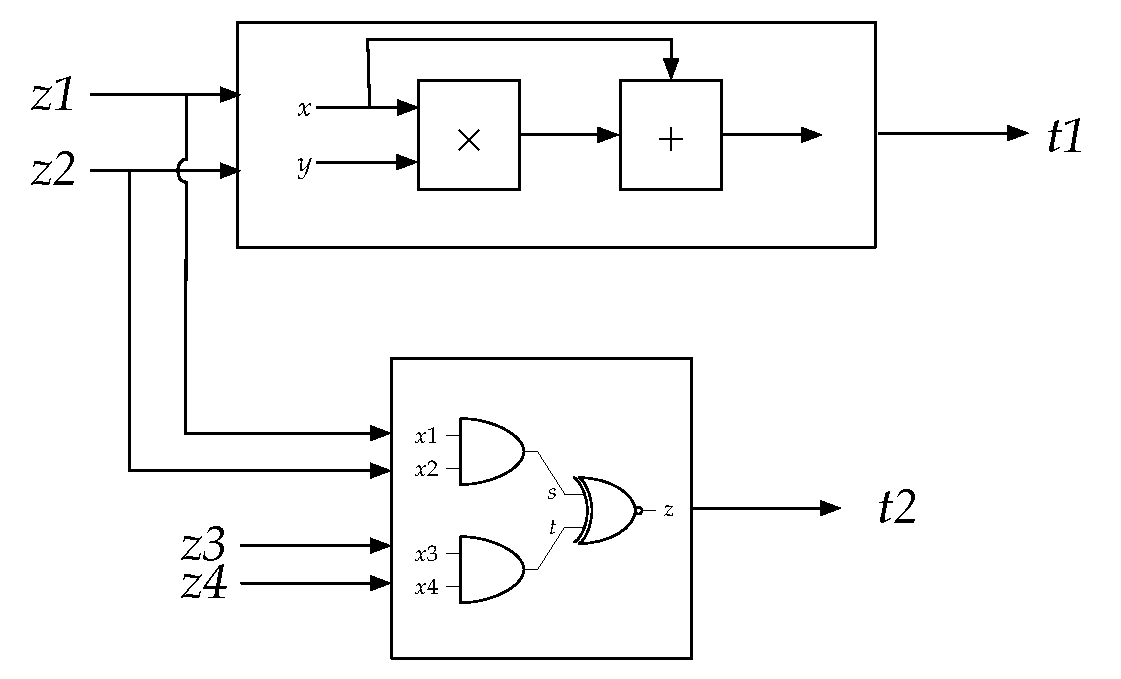
\includegraphics[width=0.9\textwidth]{images/muladdcomblogic}
\end{center}
\caption{Combination of figures \ref{fig:combinational1} and \ref{fig:muladd}.} \label{fig:combinational3}
\end{figure}


% Polymorphism
\subsubsection{Polymorphism}
The specification of a piece of digital logic is sometimes generic enough to be used in multiple ways.
The addition operation can for instance be used to add numbers regardless of their bit-representation, at least a language perspective.
When the addition operation is translated to \gls{vhdl}, a proper adder may be chosen. 
Due to the type system, we know the type of the numbers which are to be added, and as such a specific adder can be chosen.
Polymorphism makes it possible to specify and \textit{reuse} such specifications.
As an example of how code reuse is useful, consider the following code snippet, which represents the circuit of figure \ref{fig:polymorphic}.

\begin{texexptitled}[text only]{A polymorphic specification}{code:polymorphic}\begin{hscode}\SaveRestoreHook
\column{B}{@{}>{\hspre}l<{\hspost}@{}}%
\column{3}{@{}>{\hspre}l<{\hspost}@{}}%
\column{5}{@{}>{\hspre}l<{\hspost}@{}}%
\column{13}{@{}>{\hspre}l<{\hspost}@{}}%
\column{E}{@{}>{\hspre}l<{\hspost}@{}}%
\>[3]{}\Varid{commonCode}\;\Varid{f}\;\Varid{g}\;\Varid{h}\;\Varid{x}\;\Varid{y}\mathrel{=}\Varid{z3}{}\<[E]%
\\
\>[3]{}\hsindent{2}{}\<[5]%
\>[5]{}\mathbf{where}\;{}\<[13]%
\>[13]{}\Varid{z1}\mathrel{=}\Varid{f}\;\Varid{x}\;\Varid{y}{}\<[E]%
\\
\>[13]{}\Varid{z2}\mathrel{=}\Varid{g}\;\Varid{z1}{}\<[E]%
\\
\>[13]{}\Varid{z3}\mathrel{=}\Varid{h}\;\Varid{z2}\;\Varid{y}{}\<[E]%
\ColumnHook
\end{hscode}\resethooks
\end{texexptitled}

\begin{figure}[H]
\begin{center}
\centering
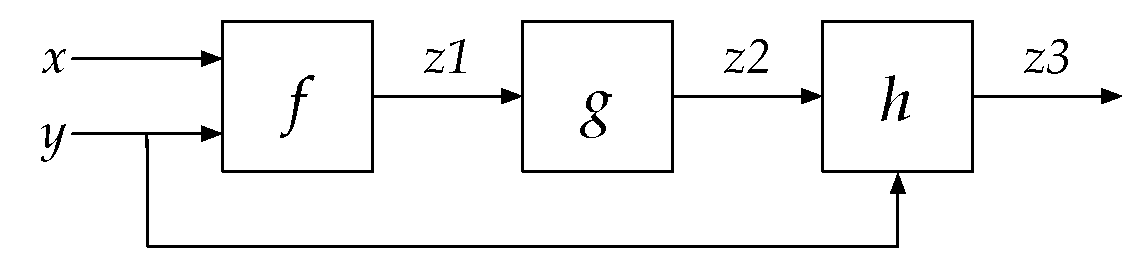
\includegraphics[width=0.8\textwidth]{images/polymorphic}
\end{center}
\caption{A polymorphic circuit, as specified by code snippet \ref{code:polymorphic}} \label{fig:polymorphic}
\end{figure}

The code of snippet \ref{code:polymorphic} only specifies in what way the functions \ensuremath{\Varid{f}},\ensuremath{\Varid{g}} and \ensuremath{\Varid{h}} interact with each other.
As the definition of \ensuremath{\Varid{commonCode}} uses the functions \ensuremath{\Varid{f}},\ensuremath{\Varid{g}} and \ensuremath{\Varid{h}} as arguments, the \ensuremath{\Varid{commonCode}} function needs to be applied to three different functions before the specification can be applied to bit-representable values.
For instance, we can use \ensuremath{\Varid{commonCode}} as 
\begin{changemargin}{1cm}{0cm}
\begin{expansionno}{text only}
\ensuremath{\Varid{specificCodeA}\mathrel{=}\Varid{commonCode}\;(\mathbin{+})\;\Varid{id}\;(\mathbin{+})}
\end{expansionno}
\end{changemargin}
or as 
\begin{changemargin}{1cm}{0cm}
\begin{expansionno}{text only}
\ensuremath{\Varid{specificCodeB}\mathrel{=}\Varid{commonCode}\;(\mathbin{*})\;\Varid{shiftL}\;(\mathbin{+})}
\end{expansionno}
\end{changemargin}
, depending on the intented usage of the \ensuremath{\Varid{commonCode}} pattern.

Both of those specifications are correct.
However, not every combination of functions leads to a correct specification.
When we use \ensuremath{\Varid{commonCode}} as in 
\begin{changemargin}{1cm}{0cm}
\begin{expansionno}{text only}
\ensuremath{\Varid{incorrectCode}\mathrel{=}\Varid{commonCode}\;(\mathbin{+})\;(\mathbin{+})\;(\mathbin{+})}
\end{expansionno}
\end{changemargin}
, then the second \ensuremath{(\mathbin{+})} function does not match with the function type which \ensuremath{\Varid{g}} is expected to have.
This is because there exists a \textit{relation} between the functions \ensuremath{\Varid{f}}, \ensuremath{\Varid{g}} and \ensuremath{\Varid{h}} within the context of the function \ensuremath{\Varid{commonCode}}.
We use \textit{type variables} to reason about these relationships.
Like value variables, type variables are referentially transparent.
For instance, the sub-expressions of \ensuremath{\Varid{commonCode}} have the following types:
\begin{changemargin}{1cm}{0cm}
\begin{expansionno}{text only}
\begin{hscode}\SaveRestoreHook
\column{B}{@{}>{\hspre}l<{\hspost}@{}}%
\column{5}{@{}>{\hspre}l<{\hspost}@{}}%
\column{E}{@{}>{\hspre}l<{\hspost}@{}}%
\>[B]{}\Varid{f}{}\<[5]%
\>[5]{}\mathbin{::}\Varid{a}\to \Varid{b}\to \Varid{c}{}\<[E]%
\\
\>[B]{}\Varid{g}{}\<[5]%
\>[5]{}\mathbin{::}\Varid{c}\to \Varid{d}{}\<[E]%
\\
\>[B]{}\Varid{h}{}\<[5]%
\>[5]{}\mathbin{::}\Varid{d}\to \Varid{b}\to \Varid{e}{}\<[E]%
\\
\>[B]{}\Varid{z1}{}\<[5]%
\>[5]{}\mathbin{::}\Varid{c}{}\<[E]%
\\
\>[B]{}\Varid{z2}{}\<[5]%
\>[5]{}\mathbin{::}\Varid{d}{}\<[E]%
\\
\>[B]{}\Varid{z3}{}\<[5]%
\>[5]{}\mathbin{::}\Varid{e}{}\<[E]%
\ColumnHook
\end{hscode}\resethooks
\end{expansionno}
\end{changemargin}
The type variables express the relation between the types of the expressions used in \ensuremath{\Varid{commonCode}}.
As \ensuremath{\Varid{f}} provides the input to \ensuremath{\Varid{g}}, the type of the input to \ensuremath{\Varid{g}} is necessarily the same as the type of the output of \ensuremath{\Varid{f}}.
The types of the remaining expressions are similarly limited.

Polymorphic types have a limitation however.
Since polymorphic types represent a range of possible representations, we can not generate hardware from a polymorphic description.
Thus, the final compilation must have fully determined types.

%%%%
% Combinational Logic and Time
%%%%
\subsection{Combinational Logic and Time}
In reality it takes time for outputs of combinational logic to become stable after a change occurs at the inputs of the circuit.
However, in synchronous hardware design this delay cannot be observed.
When the input changes, the output changes in the same timeframe.
Even though verification of time-dependent behaviour is not useful for combinational logic, the distinction between combinational logic and sequential logic still has to be made.
For this reason, the relation between inputs and outputs in combinational logic is made explicit by naming the moments at which values should exist.
To do so, we introduce time variables.
We use variables since we do not yet know at which specific time the input changes, but we would like to reason about the relation between input and output in terms of time.

Through the type system, we already have access to type information about the values used in expressions.
From the \ensuremath{\Varid{combLogic}} definition we know that \ensuremath{\Varid{combLogic}} is a function.
However, we also know that \ensuremath{\Varid{x1}} to \ensuremath{\Varid{x4}} are values with type \ensuremath{\Conid{Bit}}.
Similarly, we know the output value is of type \ensuremath{\Conid{Bit}} as well.
If we assume the output changes at moment \ensuremath{\Varid{t}}, then the input values must have stabilised at moment \ensuremath{\Varid{t}} as well.
We represent that as part of the type ascription by annotating each datatype with the same time variable as follows:
\begin{changemargin}{1cm}{0cm}
\begin{expansionno}{text only}
\ensuremath{\Varid{combLogic}\mathbin{::}\Conid{Bit}\langle\Varid{t}\rangle\to \Conid{Bit}\langle\Varid{t}\rangle\to \Conid{Bit}\langle\Varid{t}\rangle\to \Conid{Bit}\langle\Varid{t}\rangle\to \Conid{Bit}\langle\Varid{t}\rangle}
\ensuremath{\Varid{combLogic}\;\Varid{x1}\;\Varid{x2}\;\Varid{x3}\;\Varid{x4}\mathrel{=}\mathbin{...}}
\end{expansionno}
\end{changemargin}

In the above example we have defined every value to be available at the same moment in time, as is expected of combinational logic in synchronous hardware designs.
In synchronous hardware design we can always combine as much combinational logic as we wish, without having any impact on its \textit{modelled} time-dependent behaviour.
By adding more combinational logic, the time-dependent behaviour of the circuit stays the same, even though in reality, the performance suffers.

%%%%%%%%%%%%%%%%%%
%
% Sequential Logic
%
%%%%%%%%%%%%%%%%%%
\section{Specification of Sequential Logic}
Unlike combinational logic, sequential logic can not be described directly by pure functions.
Pure functions relate the output directly in terms of the input(s).
In sequential logic however, the current output does not solely depend on current input(s), but also on past input(s).
In this section we discuss how sequential logic is currently specified in \gls{clash}.
Next, we introduce how we can use time variables to specify time-dependent behaviour.
To do so, we focus on individual memory elements before defining a pipelined circuit.
Following pipelining, we discuss type (re)construction of compositions.
Finally, we discuss bounded sequences.

So far we have only shown how \gls{clash} represents combinational logic using pure functions.
Since pure functions are side-effect free, pure functions alone cannot be used to recall information from the past.
As a result, sequential logic in \gls{clash} is first defined as a pure function with a \textit{specific} type of type.
The pure function is then transformed into a component through a primitive function called \ensuremath{\Varid{lift}}, a process which is explained in greater detail later.
In this specific type of pure function, only combinational logic is defined, while sequential logic is solely represented via its inputs and outputs.

Code snippet \ref{code:sequentiallogic} shows the pattern which must be used to specify sequential logic.
As before, there is a immediate relationship between the code presented in code snippet \ref{code:sequentiallogic} and the circuit of figure \ref{fig:sequential}.

\begin{texexptitled}[text only]{Sequential logic in \gls{clash}}{code:sequentiallogic}\begin{hscode}\SaveRestoreHook
\column{B}{@{}>{\hspre}l<{\hspost}@{}}%
\column{3}{@{}>{\hspre}l<{\hspost}@{}}%
\column{5}{@{}>{\hspre}l<{\hspost}@{}}%
\column{13}{@{}>{\hspre}l<{\hspost}@{}}%
\column{19}{@{}>{\hspre}l<{\hspost}@{}}%
\column{E}{@{}>{\hspre}l<{\hspost}@{}}%
\>[3]{}\Varid{sequential}\mathbin{::}\Conid{State}\;\Varid{a}\to \Varid{b}\to (\Conid{State}\;\Varid{a},\Varid{c}){}\<[E]%
\\
\>[3]{}\Varid{sequential}\;(\Conid{State}\;\Varid{s})\;\Varid{x}\mathrel{=}(\Conid{State}\;\Varid{s'},\Varid{out}){}\<[E]%
\\
\>[3]{}\hsindent{2}{}\<[5]%
\>[5]{}\mathbf{where}\;{}\<[13]%
\>[13]{}\Varid{s'}{}\<[19]%
\>[19]{}\mathrel{=}\mathbin{...}{}\<[E]%
\\
\>[13]{}\Varid{out}{}\<[19]%
\>[19]{}\mathrel{=}\mathbin{...}{}\<[E]%
\ColumnHook
\end{hscode}\resethooks
\end{texexptitled}

The definition of \ensuremath{\Varid{sequential}} shows the type of the pure function used to describe sequential logic.
The first argument named \ensuremath{\Varid{s}} represents the input value from sequential logic of the \textit{current clockcycle}.
To distinguish between the inputs of sequential logic, and inputs of the component itself, the \ensuremath{\Conid{State}} keyword is used. 
The \ensuremath{\Conid{State}} keyword is \gls{clash} specific, and only has meaning in this specific type of function type.
In Haskell, \ensuremath{\Conid{State}} is a normal type constructor, whereas in \gls{clash} it is a reserved word.
To supply sequential logic with external input the second argument, named \ensuremath{\Varid{x}}, is used.
Using the variables \ensuremath{\Varid{s}} and \ensuremath{\Varid{x}}, the output \ensuremath{\Varid{out}} and the value of \ensuremath{\Varid{s}} in the \textit{next} clockcycle can be determined.
As a result, the input and output are synchronised to a clock, even though the specification of sequential logic does not specify the clock signal directly.
Instead, the relation between the input and the output of sequential logic is defined within the context of a single clock cycle.

\begin{figure}[H]
\begin{center}
\centering
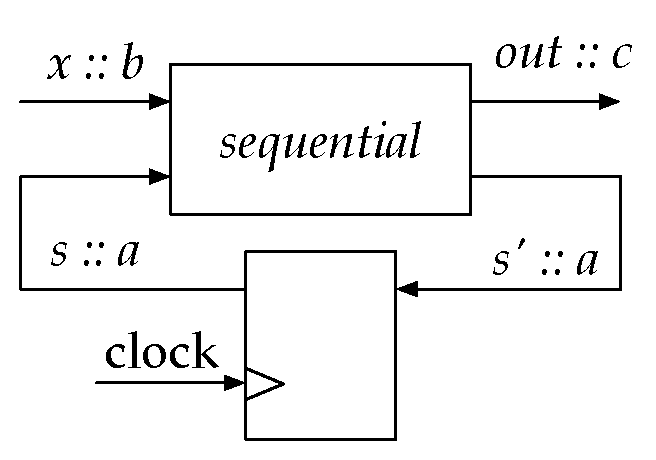
\includegraphics[width=0.5\textwidth]{images/sequential}
\end{center}
\caption{Sequential logic.} \label{fig:sequential}
\end{figure}

%%%%
% Individual Memory Elements
%%%%
\subsection{Individual Memory Elements}
Although the definition of sequential logic in \gls{clash} is flexible enough to specify feedback, we focus on a more simplified example first.
Code snippet \ref{code:singlemem} shows how a single memory element can be defined in \gls{clash}.
Like before, there exists an immediate relationship between the code and the circuit it represents.
In this example, a single type variable is enough to fully describe its behaviour.

\begin{texexptitled}[text only]{A single memory element in \gls{clash}}{code:singlemem}\begin{hscode}\SaveRestoreHook
\column{B}{@{}>{\hspre}l<{\hspost}@{}}%
\column{3}{@{}>{\hspre}l<{\hspost}@{}}%
\column{5}{@{}>{\hspre}l<{\hspost}@{}}%
\column{13}{@{}>{\hspre}l<{\hspost}@{}}%
\column{19}{@{}>{\hspre}l<{\hspost}@{}}%
\column{E}{@{}>{\hspre}l<{\hspost}@{}}%
\>[3]{}\Varid{singleMem}\mathbin{::}(\Conid{State}\;\Varid{a})\to \Varid{a}\to (\Conid{State}\;\Varid{a},\Varid{a}){}\<[E]%
\\
\>[3]{}\Varid{singleMem}\;(\Conid{State}\;\Varid{s})\;\Varid{x}\mathrel{=}(\Conid{State}\;\Varid{s'},\Varid{out}){}\<[E]%
\\
\>[3]{}\hsindent{2}{}\<[5]%
\>[5]{}\mathbf{where}\;{}\<[13]%
\>[13]{}\Varid{s'}{}\<[19]%
\>[19]{}\mathrel{=}\Varid{x}{}\<[E]%
\\
\>[13]{}\Varid{out}{}\<[19]%
\>[19]{}\mathrel{=}\Varid{s}{}\<[E]%
\ColumnHook
\end{hscode}\resethooks
\end{texexptitled}

%\begin{figure}[H]
%\begin{center}
%\centering
%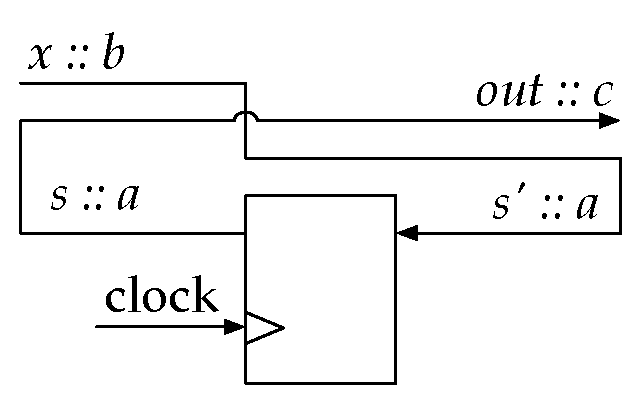
\includegraphics[width=0.5\textwidth]{images/singlememory}
%\end{center}
%\caption{A single memory element in \gls{clash}.} \label{fig:singlememory}
%\end{figure}

The same behaviour is modelled more concisely in our type system.
As shown, the definition of \ensuremath{\Varid{singleMem}} delays the input \ensuremath{\Varid{x}} with one cycle of the clock.
Delaying a value with one clockcycle implies some form of transformation in the time domain.
Instead of specifying the input and output of sequential logic separately, we directly encode this transformation in the type of the function.
As shown by code snippet \ref{code:singlememvar}, the intent of the specification which uses time variables is clear from the type of the function alone.
The input exists at time \ensuremath{\Varid{t}}, and the output exists one cycle later, at \ensuremath{\Varid{t}\mathbin{+}\mathrm{1}}.

\begin{texexptitled}[text only]{A single memory element defined using a time variable.}{code:singlememvar}\begin{hscode}\SaveRestoreHook
\column{B}{@{}>{\hspre}l<{\hspost}@{}}%
\column{3}{@{}>{\hspre}l<{\hspost}@{}}%
\column{E}{@{}>{\hspre}l<{\hspost}@{}}%
\>[3]{}\Varid{singleMem'}\mathbin{::}\Varid{a}\langle\Varid{t}\rangle\to \Varid{a}\langle\Varid{t}\mathbin{+}\mathrm{1}\rangle{}\<[E]%
\\
\>[3]{}\Varid{singleMem'}\;\Varid{x}\mathrel{=}\Varid{x}{}\<[E]%
\ColumnHook
\end{hscode}\resethooks
\end{texexptitled}

Instead of introducing temporal transformations at the term level, we introduce such transformations as part of the type. 
A memory element behaves as the identity function in the value domain, and as a linear transformation in the time-domain.
Variables on the term level are referentially transparent; they can be replaced by the same value throughout the expression without changing the behaviour of the function.
This is true when applying a positive shift to the time-domain of a value as well.
When a value exists at some point in time \ensuremath{\Varid{t}}, it can always be stored to be available at \ensuremath{\Varid{t}\mathbin{+}\Varid{a}}, where \ensuremath{\Varid{a}} is any natural number.
Specifying the time-dependent behaviour as part of the function type leads to a clean separation between \textit{what} ought to be done by a function, and \textit{when} it ought to be done.

Memory elements defined in this way have limitations however.
Memory elements which have some conditional behaviour cannot be expressed solely by transformations in the time domain.
To describe such memory elements, either a language primitive needs to be added, or the needed type of memory element should be detected from contextual information during translation to \gls{vhdl} or during hardware synthesis.

Similarly to \gls{clash}, the clock is not explicitly defined.
Even so, a relation between the time variable \ensuremath{\Varid{t}}, the expression \ensuremath{\Varid{t}\mathbin{+}\mathrm{1}} and the clock exists, as shown by figure \ref{fig:clock}.

\begin{figure}[H]
\begin{center}
\centering
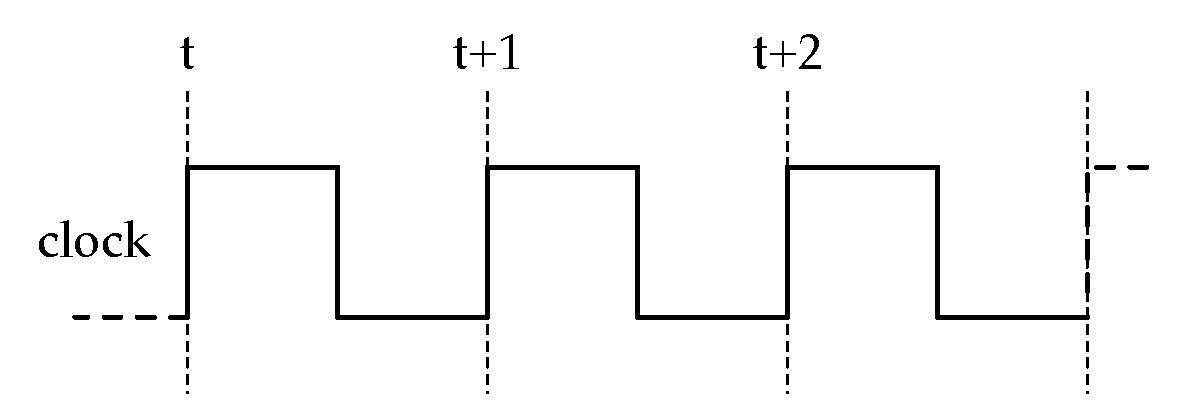
\includegraphics[width=0.6\textwidth]{images/clock}
\end{center}
\caption{Relation between the clock and time variables} \label{fig:clock}
\end{figure}

Time variables represent specific moments in ``real'' time.
However, time is discrete and as such we cannot distinguish between two moments in time which occur between $t$ and $t + 1$.
In synchronous logic, a period of time needs to pass in order for signals to stabilise.
The moment in time \ensuremath{\Varid{t}} represents the first moment when its input is stable.
The time expression \ensuremath{\Varid{t}\mathbin{+}\mathrm{1}} as part of the output defines when this output will stabilise, in relation to its input.

Similarly to the definition of \ensuremath{\Varid{singleMem}}, we can define two memory elements by changing the offset, as shown by code snippet \ref{code:doublememvar}.
\begin{texexptitled}[text only]{Two memory elements defined using a time variable.}{code:doublememvar}\begin{hscode}\SaveRestoreHook
\column{B}{@{}>{\hspre}l<{\hspost}@{}}%
\column{3}{@{}>{\hspre}l<{\hspost}@{}}%
\column{E}{@{}>{\hspre}l<{\hspost}@{}}%
\>[3]{}\Varid{doubleMem}\mathbin{::}\Varid{a}\langle\Varid{t}\rangle\to \Varid{a}\langle\Varid{t}\mathbin{+}\mathrm{2}\rangle{}\<[E]%
\\
\>[3]{}\Varid{doubleMem}\;\Varid{x}\mathrel{=}\Varid{x}{}\<[E]%
\ColumnHook
\end{hscode}\resethooks
\end{texexptitled}

We compose \ensuremath{\Varid{doubleMem}} with \ensuremath{\Varid{singleMem}} to create \ensuremath{\Varid{tripleMem}}.
The type system can infer the correct type of the composition.
As a result, the type of 
\begin{changemargin}{1cm}{0cm}
\begin{expansionno}{text only}
\ensuremath{\Varid{tripleMem}\mathrel{=}\Varid{doubleMem}\mathbin{\circ}\Varid{singleMem}}
\end{expansionno}
\end{changemargin}
is inferred to be \ensuremath{\Varid{a}\langle\Varid{t}\rangle\to \Varid{a}\langle\Varid{t}\mathbin{+}\mathrm{3}\rangle}.

Even though the hardware specifications so far have always used the same time variable, time variables are not shared between specifications.
Time variables only exist within the scope of the specification where they are introduced.
As a result, the time variable used in \ensuremath{\Varid{singleMem}} is different from the time variable used in \ensuremath{\Varid{doubleMem}}, even though they use the same identifier.

%%%%
% Pipelining
%%%%
\subsection{Pipelining}
The definition of a single memory element is straightforward in \gls{clash} as is, so it may be hard to see exactly how adding time-dependent behaviour can be advantageous based on the examples from the previous section.
To show how adding time-dependent behaviour to the type system can lead to more concise specifications, consider the following circuit.

\begin{figure}[H]
\begin{center}
\centering
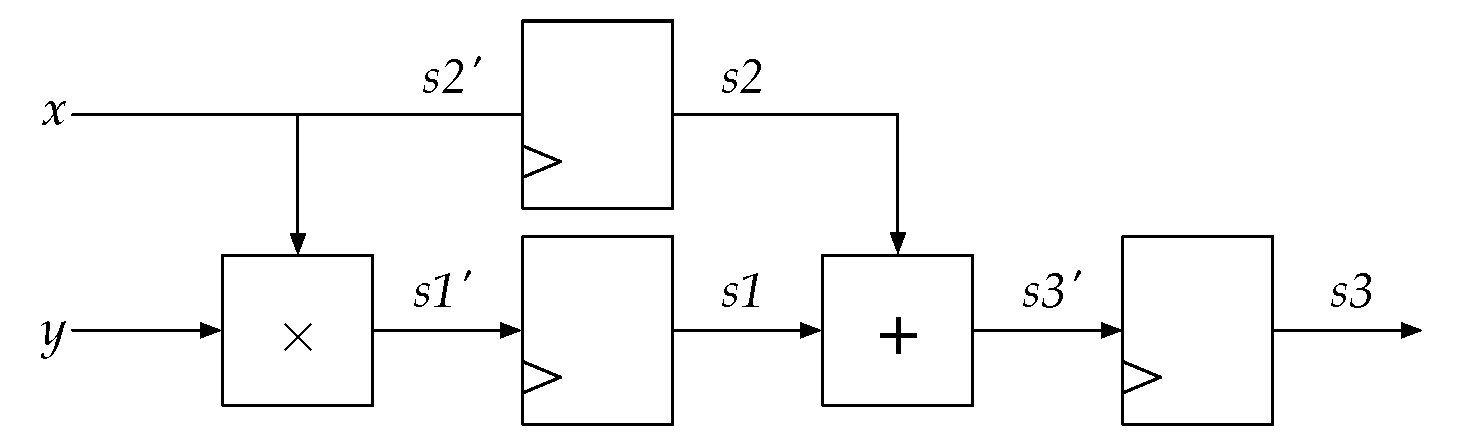
\includegraphics[width=\textwidth]{images/pipeline}
\end{center}
\caption{A pipelined circuit} \label{fig:pipeline}
\end{figure}

\gls{clash} is able to represent the circuit as a single pure function as shown by code snippet \ref{code:pipeline}.
The \ensuremath{\Conid{State}} keyword, together with the structure of the function type, allows us to transfer values between two clockcycles.
The variables \ensuremath{\Varid{s1},\Varid{s2},\Varid{s3}} represent the outputs from the registers, as opposed to the variables \ensuremath{\Varid{s1'},\Varid{s2'},\Varid{s3'}}, which represent the inputs of the registers.
This means that, given a definition of \ensuremath{\Varid{s1'}} at some clockcycle \ensuremath{\Varid{t}}, then \ensuremath{\Varid{s1}} has the same value as \ensuremath{\Varid{s1'}} at some clockcycle \ensuremath{\Varid{t}\mathbin{+}\mathrm{1}}.
This relation is straightforward, but when many registers are added, the function definitions soon become complex. 

\begin{texexptitled}[text only]{Definition of a pipeline in \gls{clash}.}{code:pipeline}\begin{hscode}\SaveRestoreHook
\column{B}{@{}>{\hspre}l<{\hspost}@{}}%
\column{3}{@{}>{\hspre}l<{\hspost}@{}}%
\column{6}{@{}>{\hspre}l<{\hspost}@{}}%
\column{13}{@{}>{\hspre}l<{\hspost}@{}}%
\column{38}{@{}>{\hspre}l<{\hspost}@{}}%
\column{E}{@{}>{\hspre}l<{\hspost}@{}}%
\>[3]{}\Varid{pipeline}\mathbin{::}\Conid{State}\;(\Conid{Int},\Conid{Int},\Conid{Int})\to (\Conid{Int},\Conid{Int})\to (\Conid{State}\;(\Conid{Int},\Conid{Int},\Conid{Int}),\Conid{Int}){}\<[E]%
\\
\>[3]{}\Varid{pipeline}\;(\Conid{State}\;(\Varid{s1},\Varid{s2},\Varid{s3}))\;(\Varid{x},\Varid{y}){}\<[38]%
\>[38]{}\mathrel{=}(\Conid{State}\;(\Varid{s1'},\Varid{s2'},\Varid{s3'}),\Varid{s3}){}\<[E]%
\\
\>[3]{}\hsindent{3}{}\<[6]%
\>[6]{}\mathbf{where}\;{}\<[13]%
\>[13]{}\Varid{s1'}\mathrel{=}\Varid{x}\mathbin{*}\Varid{y}{}\<[E]%
\\
\>[13]{}\Varid{s2'}\mathrel{=}\Varid{x}{}\<[E]%
\\
\>[13]{}\Varid{s3'}\mathrel{=}\Varid{s1}\mathbin{+}\Varid{s2}{}\<[E]%
\ColumnHook
\end{hscode}\resethooks
\end{texexptitled}

Fortunately, \gls{clash} makes it possible to create better structural descriptions by lifting pure functions such as \ensuremath{\Varid{pipeline}} to the component level.
The component level, which is based on arrows\cite{hudak2003arrows}, allows us to interpret the pure function \ensuremath{\Varid{pipeline}} as an impure function with embedded state.
Although a complete introduction to component-based programming in \gls{clash} is out of the scope of this thesis, we can show the advantages and disadvantages of the approach.
Code snippet \ref{code:pipelinec} shows the structural representation of the circuit from figure \ref{fig:pipeline}.
The \ensuremath{\Varid{lift}} function, ``lifts'' a pure function to the component level.
Unfortunately, to do so, the \textit{initial} content of the memory element has to be specified when using the lifting function.
As shown by the schematic of figure \ref{fig:pipeline}, no initial values are needed for this circuit to function properly.
Without initial values, there is a latency of two clockcycles, before the circuit produces a meaningful result.

\begin{texexptitled}[text only]{Definition of a pipeline in \gls{clash} using arrows.}{code:pipelinec}\begin{hscode}\SaveRestoreHook
\column{B}{@{}>{\hspre}l<{\hspost}@{}}%
\column{3}{@{}>{\hspre}l<{\hspost}@{}}%
\column{5}{@{}>{\hspre}l<{\hspost}@{}}%
\column{22}{@{}>{\hspre}l<{\hspost}@{}}%
\column{30}{@{}>{\hspre}l<{\hspost}@{}}%
\column{E}{@{}>{\hspre}l<{\hspost}@{}}%
\>[3]{}\Varid{pipelineC}\mathrel{=}\textbf{proc}\;(\Varid{x},\Varid{y})\to \mathbf{do}{}\<[E]%
\\
\>[3]{}\hsindent{2}{}\<[5]%
\>[5]{}\Varid{s1}\leftarrow\Varid{singleMem}{}\<[22]%
\>[22]{}\mathbin{`\Varid{lift}`}{}\<[30]%
\>[30]{}\mathrm{0}\prec\Varid{x}\mathbin{+}\Varid{y}{}\<[E]%
\\
\>[3]{}\hsindent{2}{}\<[5]%
\>[5]{}\Varid{s2}\leftarrow\Varid{singleMem}{}\<[22]%
\>[22]{}\mathbin{`\Varid{lift}`}{}\<[30]%
\>[30]{}\mathrm{0}\prec\Varid{x}{}\<[E]%
\\
\>[3]{}\hsindent{2}{}\<[5]%
\>[5]{}\Varid{s3}\leftarrow\Varid{singleMem}{}\<[22]%
\>[22]{}\mathbin{`\Varid{lift}`}{}\<[30]%
\>[30]{}\mathrm{0}\prec\Varid{s1}\mathbin{+}\Varid{s2}{}\<[E]%
\\
\>[3]{}\hsindent{2}{}\<[5]%
\>[5]{}\textbf{returnA}\prec\Varid{s3}{}\<[E]%
\ColumnHook
\end{hscode}\resethooks
\end{texexptitled}

Initial values have to be supplied regardless of the method used to create sequential logic.
Even the pure function \ensuremath{\Varid{pipeline}}, has to be lifted to the component level, before translating it to \gls{vhdl}.
As shown by \ensuremath{\Varid{pipelineC}}, the component level has a different syntax when compared to the functions shown earlier.
Usage of the language is more difficult as a result, due to the added syntax to describe interactions between components and the complexity of the underlying arrows model.

When we compare this with the code of snippet \ref{code:pipeline'}, we see that specification using time variables at the type level is a more concise way to specify time-dependent behaviour.

\begin{texexptitled}[text only]{Definition of a pipeline using time variables.}{code:pipeline'}\begin{hscode}\SaveRestoreHook
\column{B}{@{}>{\hspre}l<{\hspost}@{}}%
\column{3}{@{}>{\hspre}l<{\hspost}@{}}%
\column{E}{@{}>{\hspre}l<{\hspost}@{}}%
\>[3]{}\Varid{pipeline'}\mathbin{::}\Conid{Int}\langle\Varid{t}\rangle\to \Conid{Int}\langle\Varid{t}\rangle\to \Conid{Int}\langle\Varid{t}\mathbin{+}\mathrm{2}\rangle{}\<[E]%
\\
\>[3]{}\Varid{pipeline'}\;\Varid{x}\;\Varid{y}\mathrel{=}(\Varid{x}\mathbin{*}\Varid{y})\mathbin{+}\Varid{x}{}\<[E]%
\ColumnHook
\end{hscode}\resethooks
\end{texexptitled}

Even though the presentation is fairly concise, the definition of \ensuremath{\Varid{pipeline'}} is not equal to \gls{clash}'s definition.
Given the definition of \ensuremath{\Varid{pipeline'}}, the compiler cannot determine where \textit{exactly} memory elements ought to be inserted.
Based on the supplied function type, we know that the entire expression \ensuremath{(\Varid{x}\mathbin{*}\Varid{y})\mathbin{+}\Varid{x}} has type \ensuremath{\Conid{Int}\langle\Varid{t}\mathbin{+}\mathrm{2}\rangle}, while \ensuremath{\Varid{x}} and \ensuremath{\Varid{y}} have type \ensuremath{\Conid{Int}\langle\Varid{t}\rangle}.
We know two memory elements are needed in order to make the transformation from \ensuremath{\Varid{t}} to \ensuremath{\Varid{t}\mathbin{+}\mathrm{2}} possible, but we cannot determine where these elements ought to be inserted.
Using retiming\cite{leiserson1981optimizing}, the optimal placing of memory elements can be determined.
However, that still does not give the ability to define the circuit of figure \ref{fig:pipeline}.

To do so, individual functions representing memory elements can be added.
Since our language does not support function overloading, nor the mechanisms to use a function twice, two functions need to be defined in order to fully define the circuit of figure \ref{fig:pipeline}.
If a single \ensuremath{\Varid{delay}} function is added, such as in \ensuremath{\Varid{pipeline''}} below, the time-dependent behaviour of the circuit is defined more precisely.

\begin{texexptitled}[text only]{Definition of a pipeline using time variables and a delay.}{code:pipeline''}\begin{hscode}\SaveRestoreHook
\column{B}{@{}>{\hspre}l<{\hspost}@{}}%
\column{3}{@{}>{\hspre}l<{\hspost}@{}}%
\column{E}{@{}>{\hspre}l<{\hspost}@{}}%
\>[3]{}\Varid{pipeline''}\mathbin{::}\Conid{Int}\langle\Varid{t}\rangle\to \Conid{Int}\langle\Varid{t}\rangle\to \Conid{Int}\langle\Varid{t}\mathbin{+}\mathrm{2}\rangle{}\<[E]%
\\
\>[3]{}\Varid{pipeline''}\;\Varid{x}\;\Varid{y}\mathrel{=}((\Varid{delay}\;\Varid{y})\mathbin{*}\Varid{x})\mathbin{+}\Varid{x}{}\<[E]%
\\[\blanklineskip]%
\>[3]{}\Varid{delay}\mathbin{::}\Conid{Int}\langle\Varid{t}\rangle\to \Conid{Int}\langle\Varid{t}\mathbin{+}\mathrm{1}\rangle{}\<[E]%
\\
\>[3]{}\Varid{delay}\;\Varid{x}\mathrel{=}\Varid{x}{}\<[E]%
\ColumnHook
\end{hscode}\resethooks
\end{texexptitled}

In \ensuremath{\Varid{pipeline''}}, \ensuremath{\Varid{y}} is explicitly delayed by one clock cycle before it is multiplied by \ensuremath{\Varid{x}}.
Then, assuming \ensuremath{(\mathbin{+})} represents an adder made with combinational logic, \ensuremath{\Varid{x}} must be delayed \textit{before} using it in the multiplication.
By expressing time as part of the type, in combination with retiming, we can choose the degree of specification.

The difficulty here, is to determine when the specification of some time-dependent behaviour should be subject to retiming.
This is not part of this thesis however, which is why we do not go into detail here.

\subsection{Type Reconstruction}
One of the most important aspects of our type system, is that variables are referentially transparant and only refer to single values.
This worked out for the examples \ensuremath{\Varid{pipeline'}} and \ensuremath{\Varid{singleMem'}} earlier.
In those examples, compositions were created from composing unary functions, or by composing combinational logic.
The type system can reconstruct the type of any valid composition of well-typed functions.
As an example, consider the \ensuremath{\Varid{delay}} and \ensuremath{\Varid{sel}} functions from code snippet \ref{code:possiblecomp}.

\begin{figure}[H]
\begin{center}
\centering
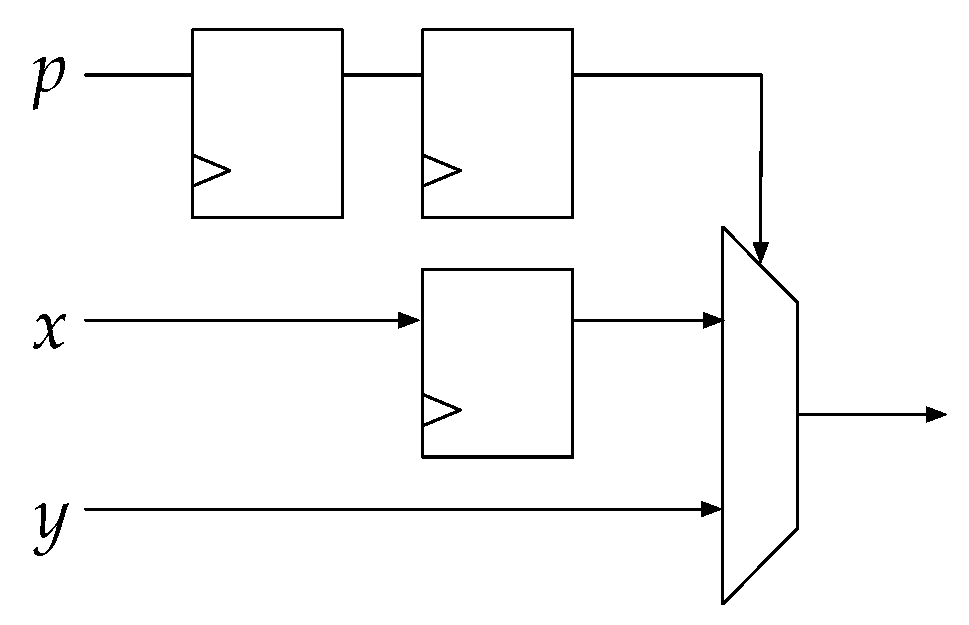
\includegraphics[width=0.6\textwidth]{images/sel}
\end{center}
\caption{Schematic representation of \ensuremath{\Varid{sel}}.} \label{fig:sel}
\end{figure}

\begin{texexptitled}[text only]{Delayed selection.}{code:possiblecomp}\begin{hscode}\SaveRestoreHook
\column{B}{@{}>{\hspre}l<{\hspost}@{}}%
\column{3}{@{}>{\hspre}l<{\hspost}@{}}%
\column{E}{@{}>{\hspre}l<{\hspost}@{}}%
\>[3]{}\Varid{sel}\mathbin{::}\Conid{Bool}\langle\Varid{t}\rangle\to \Conid{Int}\langle\Varid{t}\mathbin{+}\mathrm{1}\rangle\to \Conid{Int}\langle\Varid{t}\mathbin{+}\mathrm{2}\rangle\to \Conid{Int}\langle\Varid{t}\mathbin{+}\mathrm{2}\rangle{}\<[E]%
\\
\>[3]{}\Varid{sel}\;\Varid{p}\;\Varid{x}\;\Varid{y}\mathrel{=}\mathbf{if}\;\Varid{p}\;\mathbf{then}\;\Varid{x}\;\mathbf{else}\;\Varid{y}{}\<[E]%
\ColumnHook
\end{hscode}\resethooks
\begin{hscode}\SaveRestoreHook
\column{B}{@{}>{\hspre}l<{\hspost}@{}}%
\column{3}{@{}>{\hspre}l<{\hspost}@{}}%
\column{E}{@{}>{\hspre}l<{\hspost}@{}}%
\>[3]{}\Varid{delay}\mathbin{::}\Conid{Int}\langle\Varid{t}\rangle\to \Conid{Int}\langle\Varid{t}\mathbin{+}\mathrm{3}\rangle{}\<[E]%
\\
\>[3]{}\Varid{delay}\;\Varid{z}\mathrel{=}\Varid{z}{}\<[E]%
\ColumnHook
\end{hscode}\resethooks
\end{texexptitled}

As shown in the code, the value \ensuremath{\Varid{p}} needs to be delayed twice, in order to be used together with the value \ensuremath{\Varid{y}}.
The value \ensuremath{\Varid{x}} needs to be delayed once.
We combine the definition of \ensuremath{\Varid{sel}} with \ensuremath{\Varid{delay}} as follows:
\begin{changemargin}{1cm}{0cm}
\begin{expansionno}{text only}\begin{hscode}\SaveRestoreHook
\column{B}{@{}>{\hspre}l<{\hspost}@{}}%
\column{3}{@{}>{\hspre}l<{\hspost}@{}}%
\column{E}{@{}>{\hspre}l<{\hspost}@{}}%
\>[3]{}\Varid{comp}\;\Varid{w}\;\Varid{q}\mathrel{=}\Varid{sel}\;\Varid{q}\;\Varid{w}\;(\Varid{delay}\;\Varid{w}){}\<[E]%
\ColumnHook
\end{hscode}\resethooks
\end{expansionno}
\end{changemargin}

Through the application of \ensuremath{\Varid{sel}\;\Varid{q}} to \ensuremath{\Varid{w}}, \ensuremath{\Varid{w}} is equal to \ensuremath{\Varid{x}}.
Moreover, \ensuremath{\Varid{w}\mathrel{=}\Varid{z}} in \ensuremath{\Varid{delay}}, and \ensuremath{\Varid{z}\mathrel{=}\Varid{y}} through application of \ensuremath{\Varid{sel}}.
As a result, \ensuremath{\Varid{y}\mathrel{=}\Varid{x}}, which is seemingly impossible from the definition of \ensuremath{\Varid{sel}}.
The type of \ensuremath{\Varid{comp}} can reflect this however, by adding additional memory elements.
This is shown in figure \ref{fig:compseldelay}.

\begin{figure}[H]
\begin{center}
\centering
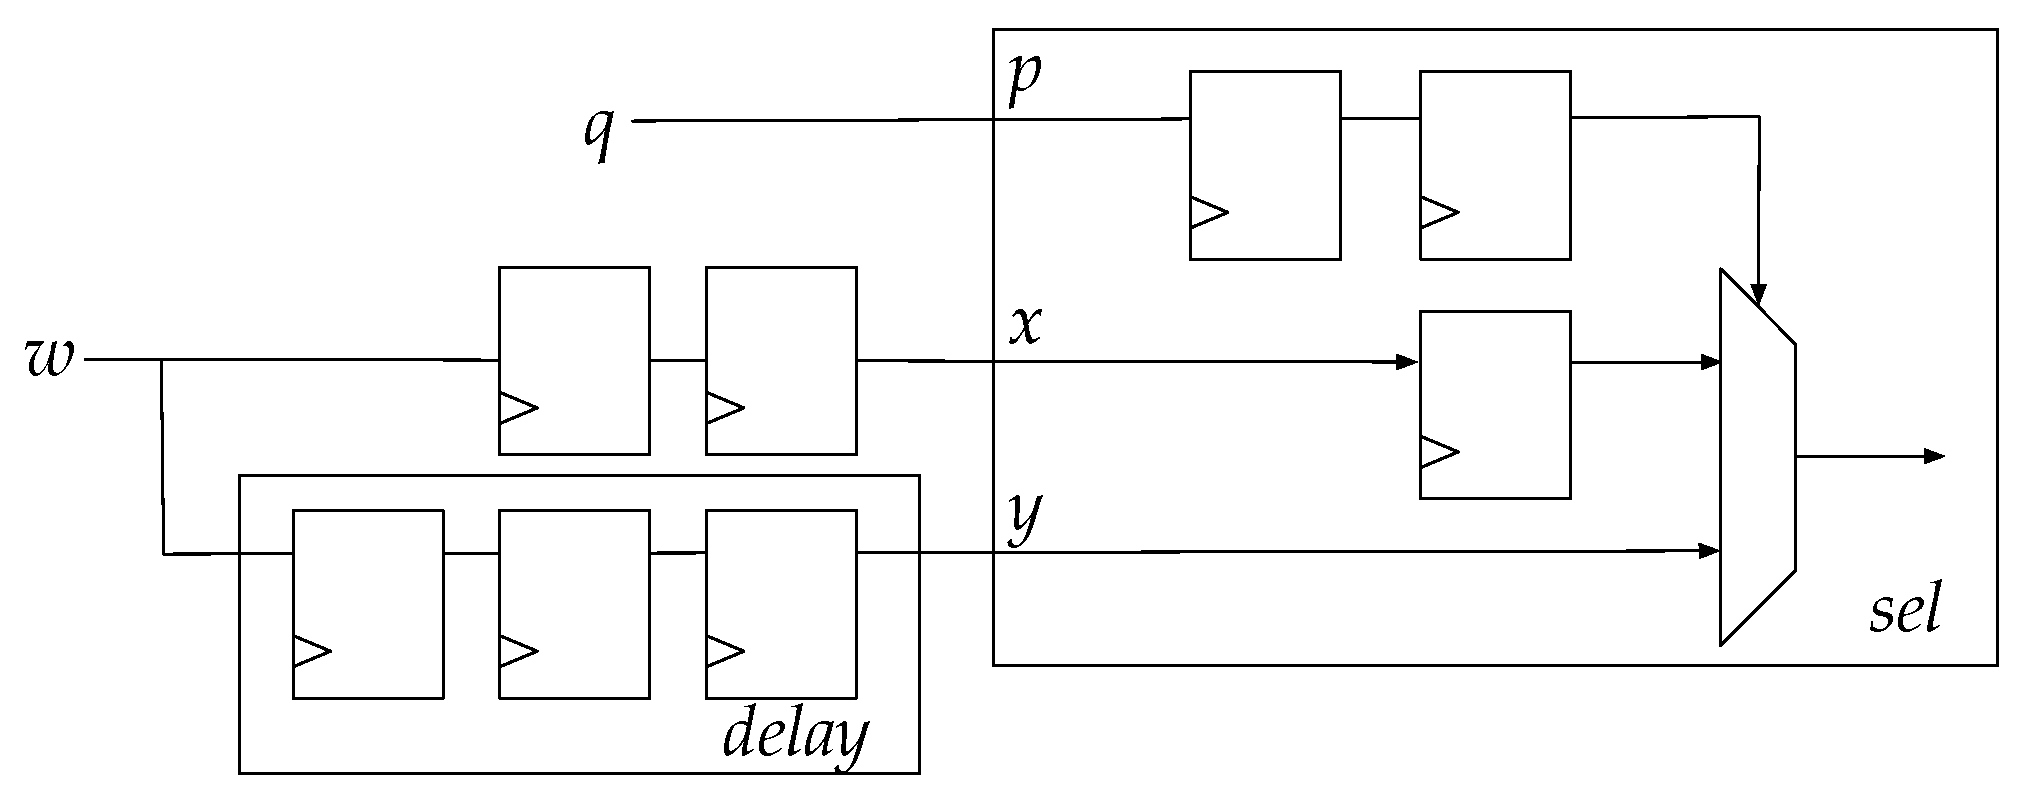
\includegraphics[width=0.9\textwidth]{images/compseldelay}
\end{center}
\caption{Schematic representation of \ensuremath{\Varid{sel}}.} \label{fig:compseldelay}
\end{figure}

As shown, two memory elements are added beyond those already available in \ensuremath{\Varid{delay}} and \ensuremath{\Varid{sel}}. 
This is done in order to equate \ensuremath{\Varid{w}} from \ensuremath{\Varid{comp}} with both \ensuremath{\Varid{x}} and \ensuremath{\Varid{y}} from \ensuremath{\Varid{sel}}.
As a result, the type of \ensuremath{\Varid{comp}} would be 
\begin{changemargin}{1cm}{0cm}
\begin{expansionno}{text only}\begin{hscode}\SaveRestoreHook
\column{B}{@{}>{\hspre}l<{\hspost}@{}}%
\column{3}{@{}>{\hspre}l<{\hspost}@{}}%
\column{E}{@{}>{\hspre}l<{\hspost}@{}}%
\>[3]{}\Varid{comp}\mathbin{::}\Conid{Int}\langle\Varid{t}\rangle\to \Conid{Bool}\langle\Varid{t}\mathbin{+}\mathrm{1}\rangle\to \Conid{Int}\langle\Varid{t}\mathbin{+}\mathrm{3}\rangle{}\<[E]%
\\
\>[3]{}\Varid{comp}\;\Varid{w}\;\Varid{q}\mathrel{=}\Varid{sel}\;\Varid{q}\;\Varid{w}\;(\Varid{delay}\;\Varid{w}){}\<[E]%
\ColumnHook
\end{hscode}\resethooks
\end{expansionno}
\end{changemargin}

There exist an odd side-effect of this automatic derivation however.
Due to how the typing rules are defined in the next chapter, functions can only be constructed where the arguments are ordered in time.
That is, a function type as \ensuremath{\Conid{Int}\langle\Varid{t}\rangle\to \Conid{Int}\langle\Varid{t}\mathbin{+}\mathrm{2}\rangle\to \Conid{Int}\langle\Varid{t}\mathbin{+}\mathrm{1}\rangle\to \Conid{Int}\langle\Varid{t}\mathbin{+}\mathrm{2}\rangle}, while seemingly valid, can not be constructed.
This side effect is most obvious when we derive the type of \ensuremath{\Varid{comp'}} below, in which the arguments \ensuremath{\Varid{w}} and \ensuremath{\Varid{q}} are flipped:
\begin{changemargin}{1cm}{0cm}
\begin{expansionno}{text only}\begin{hscode}\SaveRestoreHook
\column{B}{@{}>{\hspre}l<{\hspost}@{}}%
\column{3}{@{}>{\hspre}l<{\hspost}@{}}%
\column{E}{@{}>{\hspre}l<{\hspost}@{}}%
\>[3]{}\Varid{comp'}\mathbin{::}\Conid{Bool}\langle\Varid{t}\rangle\to \Conid{Int}\langle\Varid{t}\rangle\to \Conid{Int}\langle\Varid{t}\mathbin{+}\mathrm{3}\rangle{}\<[E]%
\\
\>[3]{}\Varid{comp'}\;\Varid{q}\;\Varid{w}\mathrel{=}\Varid{sel}\;\Varid{q}\;\Varid{w}\;(\Varid{delay}\;\Varid{w}){}\<[E]%
\ColumnHook
\end{hscode}\resethooks
\end{expansionno}
\end{changemargin}

Since arguments need to be ordered, the only way to derive a valid type from \ensuremath{\Varid{comp'}} is to add one additional register between the input to \ensuremath{\Varid{comp'}} and the input of \ensuremath{\Varid{sel}}. 

%%%%
% Sampling
%%%%
\subsection{Sequencing}
Using multiple input values which originate from the same wire is used frequently in synchronous hardware design, espcially in the area of \gls{dsp}.
We can not define such behaviour using only the syntax we have introduced earlier in this chapter, as explained in the previous section.
Consider the circuit of figure \ref{fig:sum2}, where two consecutive values are added.

\begin{figure}[H]
\begin{center}
\centering
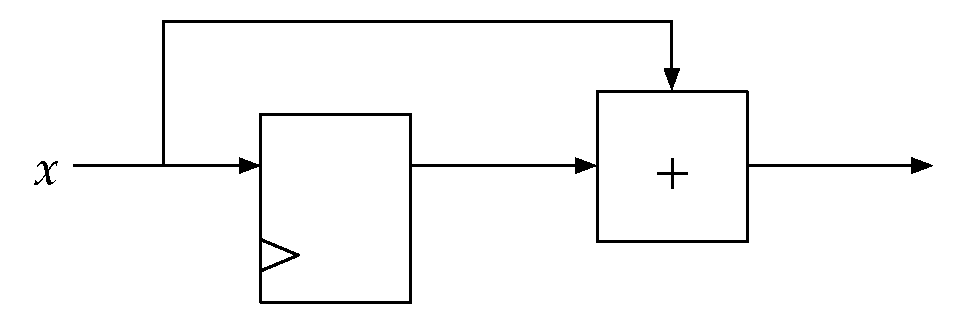
\includegraphics[width=0.6\textwidth]{images/sum2}
\end{center}
\caption{Adding two consecutive values.} \label{fig:sum2}
\end{figure}

In this schematic, \ensuremath{\Varid{x}} is not referentially transparant, as \ensuremath{\Varid{x}} refers to the wire, which represents multiple values. 
As shown in the previous section, this is not allowed in our descriptions, which makes it impossible to define this circuit directly through function abstraction and application.
Instead, we allow finite sequences of values.

\begin{texexptitled}[text only]{Summing two consecutive values.}{code:sum2}\begin{hscode}\SaveRestoreHook
\column{B}{@{}>{\hspre}l<{\hspost}@{}}%
\column{3}{@{}>{\hspre}l<{\hspost}@{}}%
\column{E}{@{}>{\hspre}l<{\hspost}@{}}%
\>[3]{}\Varid{sum2}\mathbin{::}\Conid{Int}\langle\Varid{t},\Varid{t}\mathbin{+}\mathrm{1}\rangle\to \Conid{Int}\langle\Varid{t}\mathbin{+}\mathrm{1}\rangle{}\<[E]%
\\
\>[3]{}\Varid{sum2}\langle\Varid{x1},\Varid{x2}\rangle\mathrel{=}\Varid{x1}\mathbin{+}\Varid{x2}{}\<[E]%
\ColumnHook
\end{hscode}\resethooks
\end{texexptitled}

In \ensuremath{\Varid{sum2}}, the first argument consists of two sequential values.
The type of first argument consists of two time variables, which match with the two identifiers \ensuremath{\Varid{x1}} and \ensuremath{\Varid{x2}}. 
By matching the identifiers with the time expressions, we show how \ensuremath{\Varid{x1}} relates to \ensuremath{\Varid{x2}}.
When this function is applied to another value, the correct \gls{vhdl} could, in principle at least, be generated.

The \ensuremath{\Varid{sum2}} function from above could similarly be represented as a binary function.
However, it can not be used in compositions in the same fashion as \ensuremath{\Varid{sum2}}.
As shown in the previous section, when \ensuremath{\Varid{sum2'}} is applied a single value twice, additional registers would be added to maintain referential transparency.

\begin{texexptitled}[text only]{Summing two consecutive values with a binary function.}{code:sum2'}\begin{hscode}\SaveRestoreHook
\column{B}{@{}>{\hspre}l<{\hspost}@{}}%
\column{3}{@{}>{\hspre}l<{\hspost}@{}}%
\column{E}{@{}>{\hspre}l<{\hspost}@{}}%
\>[3]{}\Varid{sum2'}\mathbin{::}\Conid{Int}\langle\Varid{t}\rangle\to \Conid{Int}\langle\Varid{t}\mathbin{+}\mathrm{1}\rangle\to \Conid{Int}\langle\Varid{t}\mathbin{+}\mathrm{1}\rangle{}\<[E]%
\\
\>[3]{}\Varid{sum2'}\;\Varid{x1}\;\Varid{x2}\mathrel{=}\Varid{x1}\mathbin{+}\Varid{x2}{}\<[E]%
\ColumnHook
\end{hscode}\resethooks
\end{texexptitled}

Sequences are really just a form of syntactic sugar.
In the next chapter, we show how functions of the form \ensuremath{\Varid{sum2'}} are converted to the equivalent of \ensuremath{\Varid{sum2}}.
Using a function with type
\begin{changemargin}{1cm}{0cm}
\begin{expansionno}{text only}
\ensuremath{\Varid{foo}\mathbin{::}\Varid{a}\langle\Varid{t}\rangle\to \Varid{a}\langle\Varid{t}\mathbin{+}\mathrm{1}\rangle\to \mathbin{...}\to \Varid{a}\langle\Varid{t}\mathbin{+}\Varid{n}\rangle\to \Varid{b}\langle\Varid{t}\mathbin{+}\Varid{n}\mathbin{+}\Varid{a}\rangle}
\end{expansionno}
\end{changemargin}
, we can derive the following structure including memory elements.

\begin{figure}[H]
\begin{center}
\centering
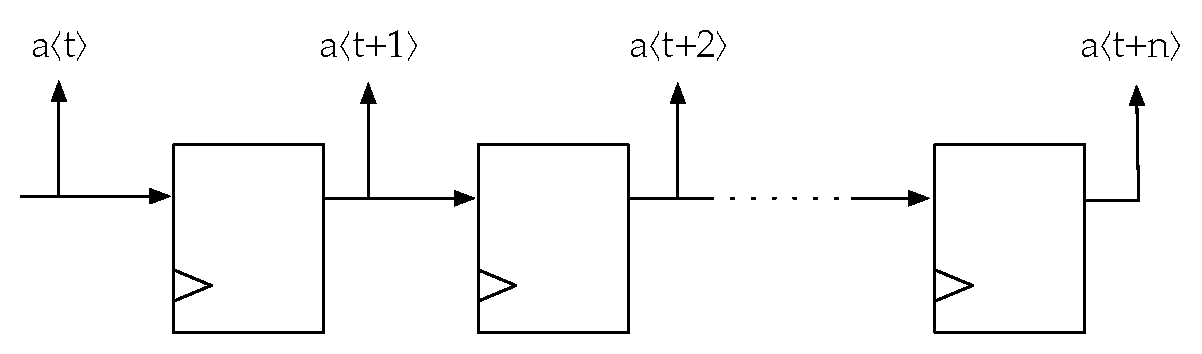
\includegraphics[width=0.8\textwidth]{images/sequence}
\end{center}
\caption{Structure generated by sequence usage.} \label{fig:sequence}
\end{figure}

The above structure only works for bit-representable values.
In a language where functions are not bit-representable, sequences can not be used for functions.

\section{Conclusion}
In this chapter we discussed the specification of time-dependent behaviour in a functional language using the type system.
One of the main advantages of the approach shown, is the fact that variables refer to \textit{individual values}.
This is different from most, if not all, existing functional hardware description languages.
In existing functional hardware description languages like Lava and \gls{forsyde}, streams are used.
In those languages, variables refer to streams of values.

In our approach, variables refer to individual values.
This is not without cost however, as variables need the ability to be moved through time.
Without the ability to be moved through time, variables which refer to individual values can not be used to describe time-dependent behaviour.
As a result from this ability, compositions of functions have a side effect.
By composing functions, additional memory elements can be added to the system.
This side-effect can be impredictable if one is not aware of its existence, which makes it less appealing to use in a hardware description language.

However, a great benefit of the expressing time-dependent behaviour in the way we showed, is that the definition of \textit{what} needs to be done is separated from \textit{when} it ought to be done.
This distinction makes it easier to reason about the time-dependent behaviour, without being concerned with what the function does, or vice versa.
By providing the ``when'' as part of the type, the time-dependent behaviour of compositions can be inferred, and checked by the system if the designer supplies the expected type.

%\subsection{Composing Sequences}
%%Before we compose various forms of sequences, it is important we point out that sequences exist \textit{solely} for specification purposes.
%%Since the time-dependent behaviour of sequences is known, we only use sequences to specify that we actually want to have access to multiple values from the same source.
%%The verification of time-dependent behaviour, which is shown later in this chapter, has nothing to do with the specification of sequences.
%%That said, 
%Composing functions which involve sequences must result in types which reflect the time-dependent behaviour of compositions.
%If compositions of functions which involve sequences do not result in types which reflect the time-dependent behaviour, then expressions cannot be guaranteed to be well-typed.
%Since well-typedness is crucial to be able to reason about time-dependent behaviour as part of the type-system, we show the resulting type of various compositions. 
%The compositions which we will discuss in this section are the following:
%\begin{itemize*}
% \item A sampling circuit composed with a single memory element.
% \item An upsampling circuit composed with a sampling circuit.
% \item A downsampling circuit composed with a sampling circuit.
% \item A downsampling circuit composed with an upsampling circuit.
%\end{itemize*}
%Even though the compositions shown above do not cover every single composition, the above scenarios are hopefully enough to (informally) prove that compositions involving sequences are indeed well-typed.
%
%\todo[inline]{Ik vraag me af of ik dit zo moet gaan doen... ik weet niet of ik hiervan wel de typing regels kan bedenken, het is veel werk en er is nog zat te doen.. Misschien er 1 of 2 uitlichtten die belangrijk zijn, en de rest future work laten?}
%
%\subsubsection{Composing sampling with memory}
%First, we compose the definition of |singleMem'| on page \pageref{code:singleMem'} with the definition of |sampling| on page \pageref{code:sampling}.
%As shown by the type of |singleMem'|, a latency of one cycle is introduced by the specification of |singleMem'|.
%For the purpose of clarification, we give every function type its own, unique time variables.
%
%\begin{changemargin}{1cm}{0cm}
%\begin{expansionno}{text only}
%|singleMem' :: Int<t1> -> <t1 + 1>|\\
%|sampling :: Int<t2..t2+2> -> Int<t2 + 2>|\\
%\\
%|samplePipe :: Int<t1..t1+2> -> <t1+3>|\\
%|samplePipe = sampling . singleMem'|
%\end{expansionno}
%\end{changemargin}
%From the type of |samplePipe|, we can see that the composition still uses sampling.
%The reverse, namely |singleMem' . sampling| has the same type, as it does not matter if a memory element is inserted before or after sampling.
%
%\subsubsection{Composing upsampling with sampling}
%\begin{changemargin}{1cm}{0cm}
%\begin{expansionno}{text only}
%|sampling :: Int<t2..t2+2> -> Int<t2+2>|\\
%|upsampling :: Int<t3> -> Int<3*t3..3*t3+2>|\\
%\\
%|sampleUp :: Int<t3> -> Int<3*t3+2>|\\
%|sampleUp = sampling . upsampling|
%\end{expansionno}
%\end{changemargin}
%
%The other way around:
%
%\begin{changemargin}{1cm}{0cm}
%\begin{expansionno}{text only}
%|upSample :: Int<t2..t2+2> -> Int<3*t2+6..3*t2+8>|\\
%|upSample = upsampling . sampling|
%\end{expansionno}
%\end{changemargin}
%
%\subsubsection{Composing downsampling with sampling}
%\begin{changemargin}{1cm}{0cm}
%\begin{expansionno}{text only}
%|sampling :: Int<t2..t2+2> -> Int<t2+2>|\\
%|downsampling :: Int<3*t4..3*t4+2> -> Int<t4+1>|\\
%\\
%|sampleDown :: Int<3*t4..3*t4+8> -> Int<t4+3>|\\
%|sampleDown = sampling . downsampling|
%\end{expansionno}
%\end{changemargin}
%
%And the other way around:
%
%\begin{changemargin}{1cm}{0cm}
%\begin{expansionno}{text only}
%|sampleDown :: Int<3*t2..3*t2+5> -> Int<t2+2>|\\
%|downSample = downsampling . sampling|
%\end{expansionno}
%\end{changemargin}
%
%\subsubsection{Composing upsampling with downsampling}
%\begin{changemargin}{1cm}{0cm}
%\begin{expansionno}{text only}
%|upsampling :: Int<t3> -> Int<3*t3..3*t3+2>|\\
%|downsampling :: Int<3*t4..3*t4+2> -> Int<t4+1>|\\
%\\
%|upDown :: Int<t4..t4+2> -> <t4+3..t4+5>|\\
%|upDown = upsampling . downsampling|
%\end{expansionno}
%\end{changemargin}
%
%Other way around:
%
%\begin{changemargin}{1cm}{0cm}
%\begin{expansionno}{text only}
%|downUp :: Int<t3> -> Int<t3+1>|\\
%|downUp = downsampling . upsampling|
%\end{expansionno}
%\end{changemargin}
%%%%%
%% Feedback
%%%%%
%\subsection{Feedback}
%%%%%
%% Verification of Composition
%%%%%
%\section{Verification of Composition}
%In this section we will explain how we use the specification of time-dependent behaviour to reason about the validity of specifications.
%Using our type-system, we know the time-dependent behaviour of individual functions.
%For instance, consider the function
%\begin{changemargin}{1cm}{0cm}
%\begin{expansionno}{text only}
%f :: Int<t'> -> Int<t'> -> Int<t'>
%f x y = x + y
%\end{expansionno}
%\end{changemargin}
%, which is a function representing combinational logic.
%
%We use it in a larger circuit, such as the one shown by figure \ref{fig:latencyverify}.
%For the purpose of explanation, we assume that the entire circuit has a single input.
%\begin{figure}[H]
%\begin{center}
%\centering
%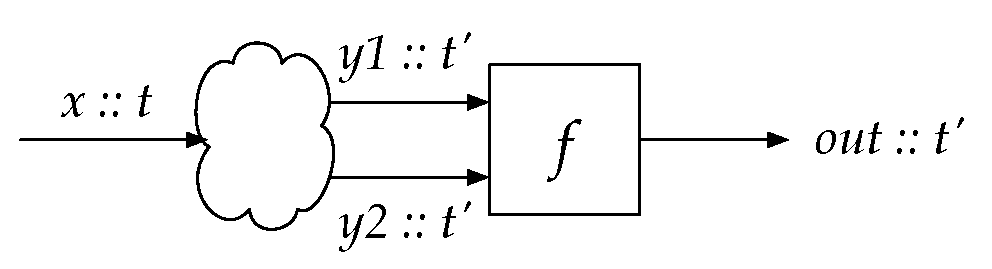
\includegraphics[width=0.6\textwidth]{images/latencyverify}
%\end{center}
%\caption{The function |f| used in a larger composition.} \label{fig:latencyverify}
%\end{figure}
%
%Whenever |f| is used in the circuit, we assume that both inputs of |f| are available at the same time.
%Moreover, both |y1| and |y2| of |f| must be subject to the same amount of latency in the entire circuit.
%This means that, when |x| occurs at |t'|, then the same number of cycles must pass between |t'| and |t|.
%Figure \ref{fig:samelatency} shows the relation between the time variable |t'|, |t| and the clock frequency.
%
%\begin{figure}[H]
%\begin{center}
%\centering
%\includegraphics[width=0.6\textwidth]{images/samelatency}
%\end{center}
%\caption{Wawa} \label{fig:samelatency}
%\end{figure}
%
%As a result, whenever we insert memory elements between |x| and |y1,y2|, the same number of memory elements ought to be inserted between |x| and |y1|, and |x| and |y2|.
%So far we have assumed implicit placement of memory elements.
%Many compositions, which are not well-typed without implicit placement, can be made to be well-typed with implicit placement of memory elements.
%
%It is also possible to use explicit placement of memory elements.
%When using explicit memory elements, other aspects of time-dependent behaviour can be verified.
%To explain the difference between these two approaches, we first discuss implicit placement of memory elements, after which we will discuss explicit placement of memory elements.
%
%\subsection{Implicit Placement of Memory Elements}
%\begin{texexptitled}[text only]{Incorrect sampling definition.}{code:incorrectsampling}
%> incorrectSampling :: Int<t,t+1,t+2> -> Int<t+1>
%> incorrectSampling <x1,x2,x3> = x1 + x2 + x3
%\end{texexptitled}
%
%\begin{figure}[H]
%\begin{center}
%\centering
%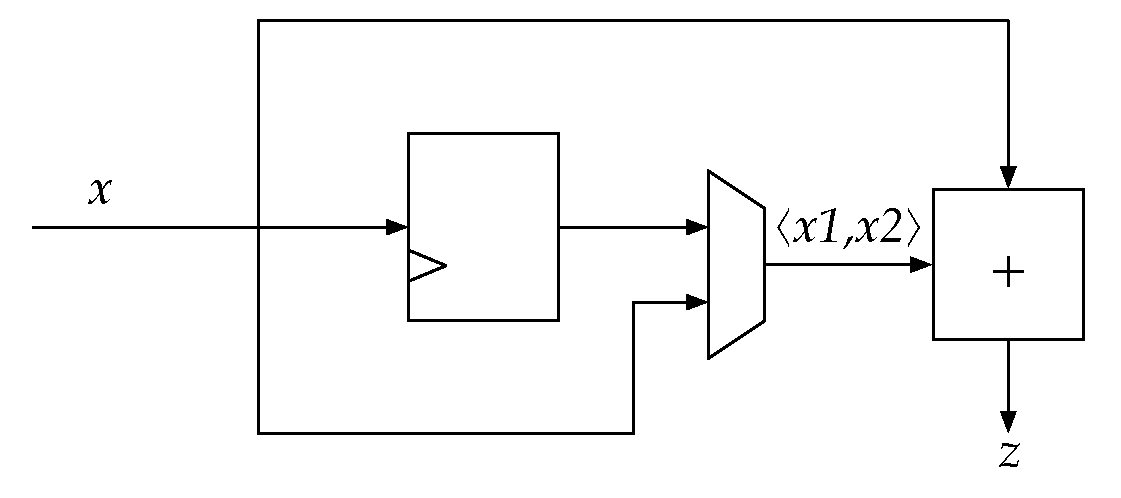
\includegraphics[width=0.6\textwidth]{images/compositioninc2}
%\end{center}
%\caption{Composition of |+|, |*| and |singleMem'|.} \label{fig:compositioninc2}
%\end{figure}
%
%\begin{texexptitled}[text only]{Correct composition.}{code:composition1cor}
%> composition'' x = z
%>   where   
%>           f :: Int<t> -> Int<2*t,2*t+1>
%>           f x   = <x,x>
%>           z     = (f x) + x
%\end{texexptitled}
%
%
%\subsection{Explicit Memory Elements}
%
%We discuss two approaches for inserting memory elements.
%The first approach is the least strict, in that \textit{any} amount of memory elements may be added to make the circuit function properly according to specification.
%So far we only defined individual functions, without reasoning about composing them.
%Individual functions can lead to incorrect specifications, as shown by the code of snippet \ref{code:incorrectsampling}.
%There, the |x3| is available at |<t+2>|, while the output is available at |<t+1>|.
%
%Since |incorrectSampling| is defined by the expression |x1 + x2 + x3|, the result of the composition can be available no sooner than |t+2|, as that is when |x3| is available.
%As a result, this specification is not well-typed.
%
%However, even when individual components are well-typed, compositions using those components do not have to be well-typed.
%In our extension of the type-system, time-dependent behaviour of individual components must always be maintained.
%For instance, when we represent combinational logic as a function with the type |Int<t> -> Int<t> -> Int<t>|, then the incurred latency for both inputs needs to be the same.
%\begin{texexptitled}[text only]{Incorrect composition.}{code:composition1inc}
%> (+) :: Int<t> -> Int<t> -> Int<t>
%> singleMem' :: Int<t> -> Int<t+1>
%> 
%> f :: Int<t> -> Int<t> -> Int<t+1>
%> f x y = (singleMem' x) + y)
%\end{texexptitled}
%
%\begin{figure}[H]
%\begin{center}
%\centering
%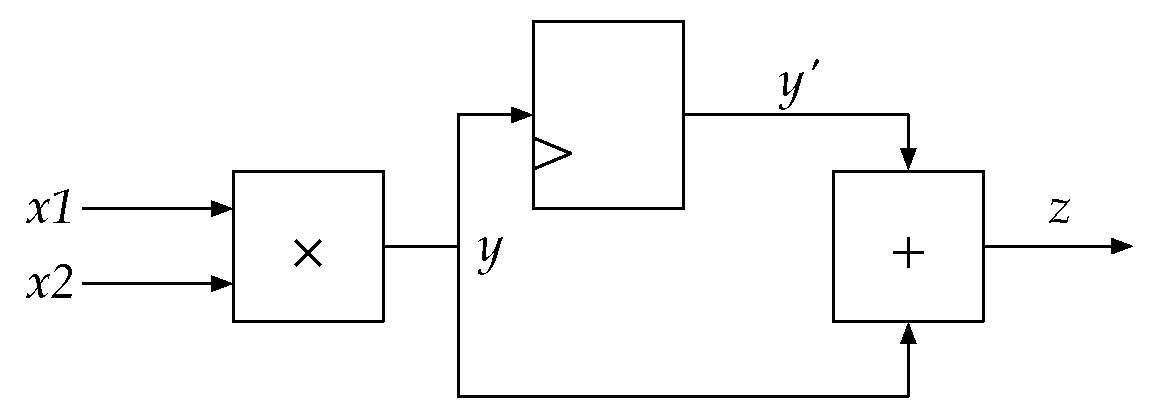
\includegraphics[width=0.6\textwidth]{images/compositioninc}
%\end{center}
%\caption{Composition of |+|, |*| and |singleMem'|.} \label{fig:compositioninc}
%\end{figure}
%
%\begin{texexptitled}[text only]{Incorrect composition.}{code:composition1inc}
%> (+) :: Int<t> -> Int<t> -> Int<t>
%> (*) :: Int<t> -> Int<t> -> Int<t>
%> singleMem' :: Int<t> -> Int<t+1>
%>
%> composition x1 x2 = 
%>   where   y   = x1 + x2
%>           y'  = singleMem' y
%>           z   = y * y'
%\end{texexptitled}
%
%\begin{texexptitled}[text only]{Correct composition.}{code:composition1cor}
%> composition' :: Int<t,t+1> -> Int<t,t+1> -> Int<t+1>
%> composition' x1 x2 = z
%>   where   y           = x1 + x2
%>           z           = f y
%>
%>           f :: Int<t,t+1> -> Int<t+1>
%>           f <y1,y2>   = y1 * y2 
%\end{texexptitled}
%
%\begin{texexptitled}[text only]{Correct composition.}{code:composition1cor}
%> composition' :: Int<t> -> Int<t> -> Int<t+1>
%> composition' x1 x2 = z
%>   where   y   = x1 + x2
%>           y'  = singleMem' y 
%>           z   = f y y'
%>
%>           f :: Int<t> -> Int<t+1> -> Int<t+1> 
%>           f   = (*)
%\end{texexptitled}

%In this chapter we will focus mainly on expressing timing constraints in source code.
%First we will briefly introduce basic syntax, operator precedence and type constructor precedence.
%Afterwards we will give a combined representation for type and time ascription, as well as providing a method to encode sequences as function arguments.
%Finally we will introduce some specific notation in creating feedback structures, as well as describing syntax which allows interactivity.
%
%Even though syntax is usually defined in pure ASCII form, we chose to typeset a few tokens to increase the readability.
%For instance, the |"->"| token is represented as $\rightarrow$, while angled brackets |"<"| \& |">"| are typeset as $\langle$ \& $\rangle$.
%
%\section{Basic Syntax}
%Since the semantics of our type-inference algorithm uses the $\lambda$-calculus, an obvious starting point for discussion of syntax are function definitions.
%Using let bindings we can introduce functions which are used multiple times within a single expression.
%When consider the top-level of a functional program, it generally consists of multiple functions used in different parts of the program.
%Each function has an identifier, which is simply a named variable of the $\lambda$-calculus.
%For instance, when we refer to the function |id x = x|, then |id| is variable name within a certain scope, which represents a function with type |X -> X|.
%The definition of |id x = x| represents $\lambda$-abstraction in the $\lambda$ calculus in the form of $id = \lambda x.x$.
%
%We can represent top-level functions by using nested let-bindings. 
%For instance, the code 
%\begin{changemargin}{1cm}{0cm}
%\begin{expansionno}{text only}%{On the $\lambda$-calculus}{exp:lambda}
%\begin{code}
%foo x = x + x
%
%bar x = x * x
%
%main x  =   let   y = foo x
%            in    bar y
%\end{code}
%\end{expansionno}
%\end{changemargin}
%could be translated to a \textit{nested} let-binding as follows
%\begin{changemargin}{1cm}{0cm}
%\begin{expansionno}{text only}%{On the $\lambda$-calculus}{exp:lambda}
%\begin{code}
%main x  =   let foo x = x + x
%            in  let bar x = x * x
%                in  let   y = foo x
%                    in    bar y
%\end{code}
%\end{expansionno}
%\end{changemargin}
%
%This shows how top-level definitions can be translated using let-bindings when we consider let-polymorhism.
%Using the |main| function to identify the top-level function, all other functions can be translated as part of the let-binding.
%As shown, we allow \textit{shadowing} of variables, meaning we can introduce a variable using the same identifier as a variable introduced in a higher scope.
%
%Of course, the definition of |foo| might have used |bar| or vice versa.
%When |foo| uses |bar|, we must introduce |foo| in a let-binding before we can introduce |bar|.
%This means that we must figure out the proper ordering in which to introduce functions in nested let-bindings.
%The ordering can be easily derived when parsing the code however, something which we do not focus on here.
%
%While let-bindings are useful, nesting let-bindings are difficult to read when complexity of descriptions increases.
%For this purpose we can allow multiple bindings within a single scope.
%For instance, in the above code the scope of |bar| is nested one level deeper than the scope of |foo|.
%Using multiple bindings in one let-binding we can introduce |foo| and |bar| within a single scope:
%\begin{changemargin}{1cm}{0cm}
%\begin{expansionno}{text only}%{On the $\lambda$-calculus}{exp:lambda}
%\begin{code}
%main x  =   let foo x = x + x
%                bar x = x * x
%            in  let   y = foo x
%                in    bar y
%\end{code}
%\end{expansionno}
%\end{changemargin}
%
%As can be seen from the examples so far, multiple bindings within the scope of a single let-statement need us to determine which definitions belong to which scope.
%In the example above we can see that |bar| can only realistically exist in the same scope as |foo|.
%However, we must define how we can determine to which scope an expression belongs in order to parse such expressions.
%The off-side rule allows us to define when a new scope begins solely by \textit{indentation} of a term.
%For instance, in the above example foo and bar have similar amounts of indentation, meaning they belong to the same scope.
%Parsing source code which contains the off-side rule is difficult, however as we are only defining syntax here this is of no concern.
%An implementation including a parser could always revert to bracket notion for scoping, as used more imperative languages such as C.
%
%\subsection{Type Ascription}
%In Haskell, type ascription is done using the |::| operator.
%The |::| operator accepts an identifier on the left hand side, and a type on the right hand side.
%The |::| operator is essentially a function which informs the type-system on what type we expect a variable to have.
%For instance, the identity function can be \textit{restricted} to only |Int| types when ascribed with the proper type, as shown below.
%\begin{changemargin}{1cm}{0cm}
%\begin{expansionno}{text only}%{On the $\lambda$-calculus}{exp:lambda}
%\begin{code}
%id :: Int -> Int
%id x = x
%\end{code}
%\end{expansionno}
%\end{changemargin}
%
%Type ascription can also occur within a function.
%\begin{changemargin}{1cm}{0cm}
%\begin{expansionno}{text only}%{On the $\lambda$-calculus}{exp:lambda}
%\begin{code}
%main x y =  let id z = z
%            in (id x) + ((id :: Int -> Int) y)
%\end{code}
%\end{expansionno}
%\end{changemargin}
%, which shows that the type of |id|, which is |X -> X| under let-polymorphism, is restricted to |Int -> Int| for the second usage when applied to |y|.
%
%Let-polymorphism allows us to define polymorphic functions.
%However, we can also restrict polymorphism using ascription by naming the type variables.
%In Haskell this is done using lower-case letters, to distingush them from type constructors which start with a capital letter.
%Here we follow the same approach, where usage of lower-case letters in ascription automatically introduces the type variables.
%For instance, in the code
%\begin{changemargin}{1cm}{0cm}
%\begin{expansionno}{text only}%{On the $\lambda$-calculus}{exp:lambda}
%\begin{code}
%choose :: a -> a -> a -> a
%choose x y z = if z then x else y
%\end{code}
%\end{expansionno}
%\end{changemargin}
%we restrict the types of |x|, |y| and |z| to be equal, regardless what these types may be.
%Since the |if then else| statement only accepts values of the boolean type, the other arguments are similarly restricted to boolean types. 
%In Haskell type variables have limited scope; type variables are only valid within the ascription they are used in.
%In our syntax we assume type variables to behave according to the same scoping rules as regular variables.
%This means they can be \textit{shadowed} by variables in a nested scope, but are available to all nested scopes if not shadowed.
%The same behaviour is also available in Haskell through the ``ScopedTypeVariables'' extension of GHC.
%
%\subsection{Function Application and Precedence}
%As in Haskell, function can be used in an infix manner.
%When defining a function such as |++|, shown below, we would like to use it infix whenever possible.
%When we define a function such as |++|, together with its type, then the parentheses indicate that this is regarded as an infix term.
%\begin{changemargin}{1cm}{0cm}
%\begin{expansionno}{text only}%{On the $\lambda$-calculus}{exp:lambda}
%\begin{code}
%(++) :: Int -> Int -> Int
%x ++ y = x + (y + y)
%\end{code}
%\end{expansionno}
%\end{changemargin}
%
%As shown, we have not defined the associativity of application.
%Whenever we apply a function we consider the application operation to be left associative.
%In the code snippet below
%\begin{changemargin}{1cm}{0cm}
%\begin{expansionno}{text only}%{On the $\lambda$-calculus}{exp:lambda}
%\begin{code}
%foo x = x + x
%bar x = x * x
%main x = bar foo x
%\end{code}
%\end{expansionno}
%\end{changemargin}
%, |bar foo x| is interpreted as |(bar foo) x|. 
%As bar uses a multiplication operation this would give a type error, as we are trying to multiply a function with itself.
%Brackets are needed in order to indicate the exact intention.
%Here the definition of |main| would have to be changed to |main x = bar (foo x)| in order to work properly.
%
%Similarly, type constructors are right associative.
%This means that a function with type |Int -> Int -> Int| is actually interpreted as |Int -> (Int -> Int)|, meaning the result of the first application is another function.
%
%\section{Time Representation}
%In order to concisely define a function's type and timing behaviour we will first define ascription involving both time and types.
%From a semantical point of view we do not distinguish between functions and other values when discussing time constraints.
%Whenever we have a function such as |Int -> (Int -> Int)|, we can ascribe each function with a time variable.
%For instance, we could define the entire function to exist at |t|. 
%When applied to a value this creates another function, which exists at (for example) |t+1|. 
%Finally, when applied to another value the final result is available at |t+2|.
%We can relate each subsequent value with a time variable as follows:
%\begin{changemargin}{1cm}{0cm}
%\begin{expansionno}{text only}%{On the $\lambda$-calculus}{exp:lambda}
%\begin{code}
%Int -> (Int -> Int)   @ t
%Int -> Int            @ t + 1
%Int                   @ t + 2
%\end{code}
%\end{expansionno}
%\end{changemargin}
%
%In order to ascribe each individual function with this time behaviour we use the same $\langle$ and $\rangle$ brackets as we used for introducing sequences in the previous chapter.
%Using the angled brackets we can ascribe each type with a time variable.
%Since we do not distinguish between functions and other values from the timing perspective, we consider the following definition
%\begin{changemargin}{1cm}{0cm}
%\begin{expansionno}{text only}%{On the $\lambda$-calculus}{exp:lambda}
%|Int<t> -> Int<t + 1> -> Int<t+2>|
%\end{expansionno}
%\end{changemargin}
%equivalent to
%\begin{changemargin}{1cm}{0cm}
%\begin{expansionno}{text only}%{On the $\lambda$-calculus}{exp:lambda}
%|(Int -> (Int -> (Int <t+2>))<t+1>)<t>|
%\end{expansionno}
%\end{changemargin}
%
%In the latter case we ascribe every partially applied function a specific time variable.
%Whenever time variables are equivalent, as in |Int<t> -> Int<t> -> Int<t>|, then the former definition is equivalent to |(Int -> Int -> Int)<t>|.
%To distinguish between regular type ascription and the introduced combination, we introduce the |:@| operator.
%Like the |::| operator, the |:@| operator accepts a variable name on the left hand side, while accepting a type-time combination on the right hand side.
%As an example, we define a timed adder below.
%\begin{changemargin}{1cm}{0cm}
%\begin{expansionno}{text only}%{On the $\lambda$-calculus}{exp:lambda}
%\begin{code}
%f :@ Int<t> -> Int<t + 1> -> Int<t+2>
%f x y = x + y
%\end{code}
%\end{expansionno}
%\end{changemargin}
%While types and timing combinations can be used, sometimes it is only needed to ascribe terms with timing information only.
%For this we use the |@| operator which, like type ascription, can be used within an expression.
%For instance, we can explicitly define registers as introduced in the previous chapter:
%\begin{changemargin}{1cm}{0cm}
%\begin{expansionno}{text only}%{On the $\lambda$-calculus}{exp:lambda}
%\begin{code}
%foo x y =   let x' = x @ t
%            in  (x' + y) @ t + 1
%\end{code}
%\end{expansionno}
%\end{changemargin}
%, in which |foo| would be equivalent to
%\begin{changemargin}{1cm}{0cm}
%\begin{expansionno}{text only}%{On the $\lambda$-calculus}{exp:lambda}
%\begin{code}
%foo :@ Int<t> -> Int<u> -> Int<t+1>
%foo x y = x + y
%\end{code}
%\end{expansionno}
%\end{changemargin}
%, where |u =< t + 1|.
%
%\section{Sequences}
%So far we have not discussed sequences.
%In the previous chapter we hinted at having a solution for using sequences as function arguments.
%Using the same syntax as above, we can define the following sampling code:
%\begin{changemargin}{1cm}{0cm}
%\begin{expansionno}{text only}%{On the $\lambda$-calculus}{exp:lambda}
%\begin{code}
%f :@ Int<t,t+1,t+2> -> Int<t+2>
%f <x,y,z> = x + y + z
%\end{code}
%\end{expansionno}
%\end{changemargin}
%
%In this example the output is the summation of three sequential values from a single wire.
%If we define the input as a stream of values $v = v_1,v_2,\ldots,v_n$, then the output would be defined no earlier than when $v_3$ is defined.
%The earliest output of the circuit would be $v_1 + v_2 + v_3$.
%However, in the next cycle, $x = y$, $y = z$ and $z = v_4$, which means that |f| samples the input in a sequential fashion.
%As shown, we use the definition of a sequence directly in the definition of the time-dependent behaviour of |f|.
%Part of the definition is the term |<x,y,z>|, which deconstructs a sequence consisting of three variables into the individual variables.
%When we deconstruct the sequence we can relate every variable with a timing expression.
%The above code could then be transformed as if accepting 3 individual arguments as follows:
%\begin{changemargin}{1cm}{0cm}
%\begin{expansionno}{text only}%{On the $\lambda$-calculus}{exp:lambda}
%\begin{code}
%f :@ Int<t> -> Int<t+1> -> Int<t+2> -> Int<t+2>
%f x y z = x + y + z
%\end{code}
%\end{expansionno}
%\end{changemargin}
%
%Sequence construction can be done using the bracket notation as well.
%\begin{changemargin}{1cm}{0cm}
%\begin{expansionno}{text only}%{On the $\lambda$-calculus}{exp:lambda}
%\begin{code}
%f :@ Int<t> -> Int<2t,2t+1>
%f x = <x,x+42>
%\end{code}
%\end{expansionno}
%\end{changemargin}
%Here, |f| accepts a single sample, which is used in a sequence.
%Sequences introduce upsampling, where the number of elements of the sequence relates the ratio between the input and the output samples.
%Here, the output produces two samples, while using only a single input.
%
%While the above syntax to create sequences is concise enough to describe upsampling, the same syntax may be too concise when individual elements of the sequence are important.
%This is the case when we consider feedback, where distinguishing the initial value of a register can be important.
%Sequences are not first-class in our language, but we introduce syntactic sugar from which it appears as if sequences are first class.
%In let-bindings we introduce variables and definitions of variables.
%To build a sequence we allow association of a single variable within a let-binding with multiple other expressions, as shown below.
%\begin{changemargin}{1cm}{0cm}
%\begin{expansionno}{text only}%{On the $\lambda$-calculus}{exp:lambda}
%\begin{code}
%f :@ Int<t> -> Int<0,t>
%f x =   let x'  @ 0       = 42 + x
%                @ t       = x' + x
%        in x'
%\end{code}
%\end{expansionno}
%\end{changemargin}
%
%The ordering in which subsequent definitions appear in the let-binding combined with ascription also defines the ordering of the sequence.
%
